% !TEX root = acsfubAuthorGuidelines-short.tex
\usepackage{tikz}
\usetikzlibrary{positioning,calc}
\usepackage{csquotes}
\usepackage{hyperref}
\usepackage{subfigure}
\usepackage{pgfplotstable}
\pgfplotsset{compat=1.18}

\renewcommand{\sectionautorefname}{Section}
\renewcommand{\subsectionautorefname}{Section}
\renewcommand{\subsubsectionautorefname}{Section}

% ---------------------------------------------------------------------
% EG author guidelines plus sample file for EG publication using LaTeX2e input
% D.Fellner, v2.02, Jan 25, 2017


\title[Generating Spatial Coordinate Datasets from Text Embeddings]%
      {Towards On-Device Continual Learning: A Pipeline for Generating Spatial Coordinate Datasets from Text Embeddings}

% FILMUNI: for anonymous conference submission please enter your SUBMISSION ID
% instead of the author's name (and leave the affiliation blank) !!
% for final version: please provide your *own* ORCID in the brackets following \orcid; see https://orcid.org/ for more details.

% AUTHOR SECTION NOT INCLUDED IN 1ST SUBMISSION (BLIND REVIEW)
\author[P. Gerdes ]
{\parbox{\textwidth}{\centering P. Gerdes$^{1}$}
\\
{\parbox{\textwidth}{\centering $^1$Film University Babelsberg KONRAD WOLF, Germany\\} 
}
}

% KEYWORDS:
% Dataset Generation
% Dimensionality Reduction
% Continual Learning

%-------------------------------------------------------------------------
\begin{document}

\teaser{
    \centering
    \subfigure[all-MiniLM-L6-v2 UMAP]{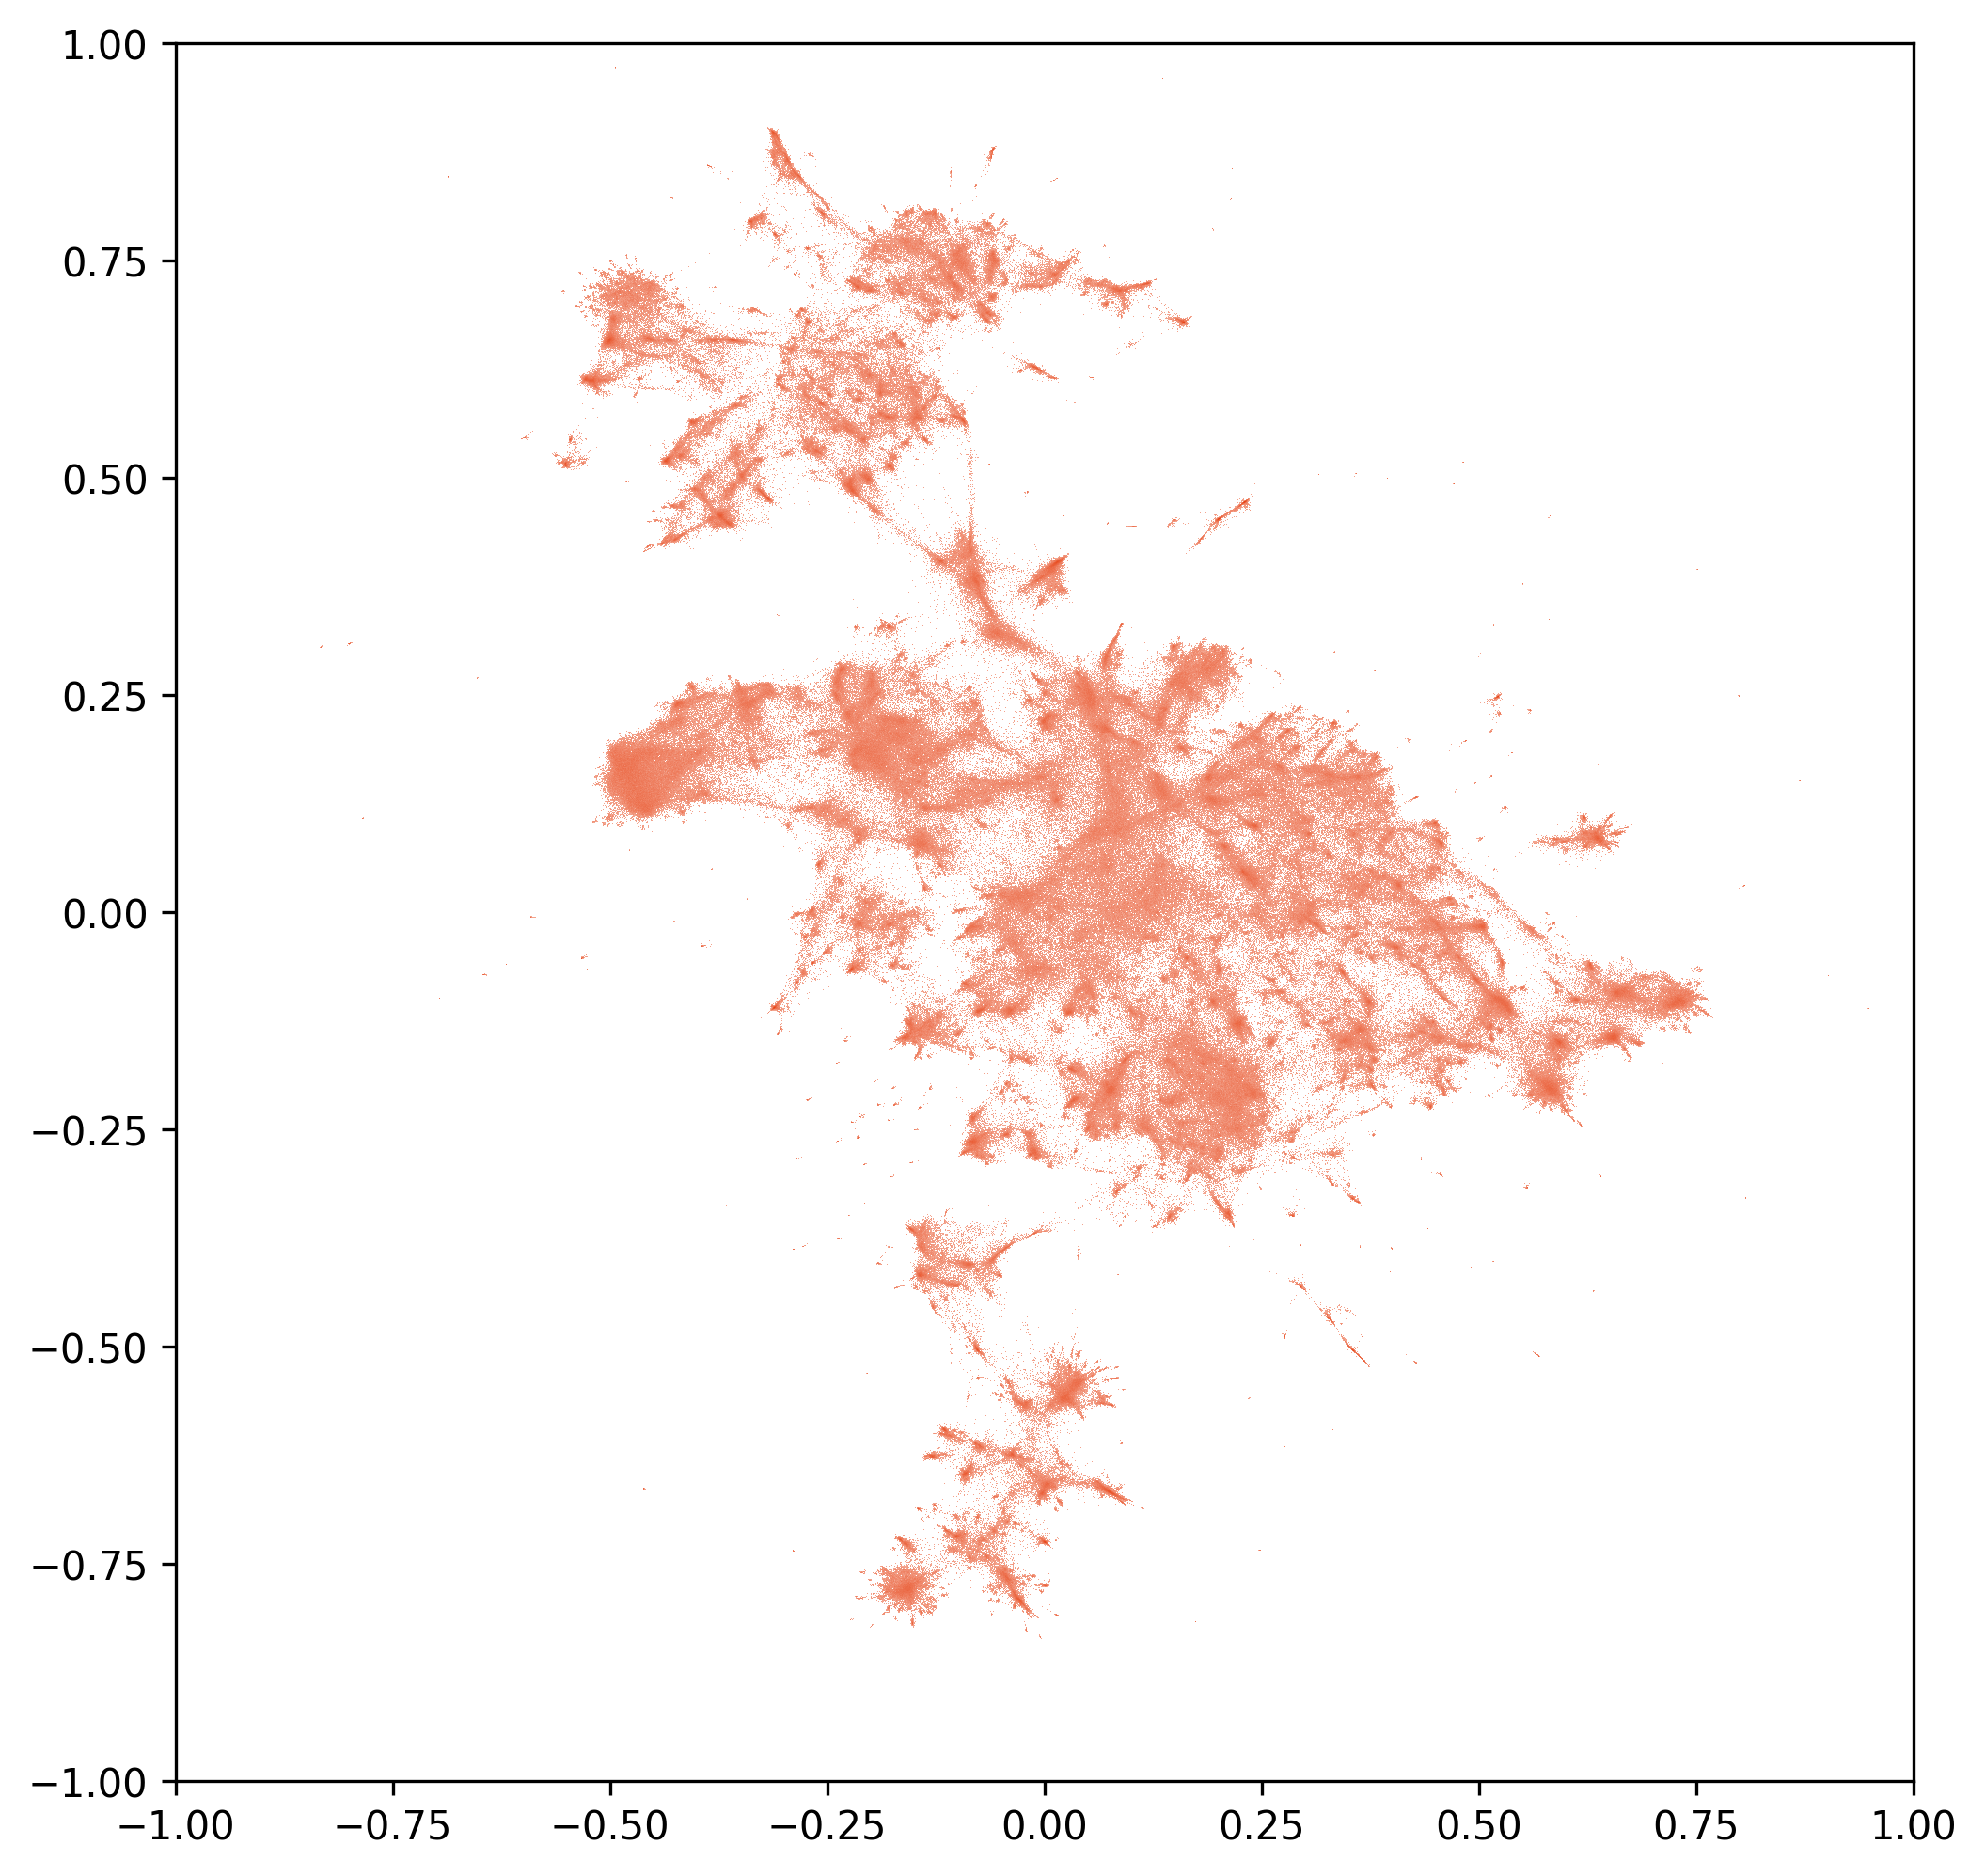
\includegraphics[width=.32\linewidth]{../src/img/all_MiniLM_L6_v2_umap.png}\label{fig:minilm-umap}}
    \hfill
    \subfigure[all-mpnet-base-v2 UMAP]{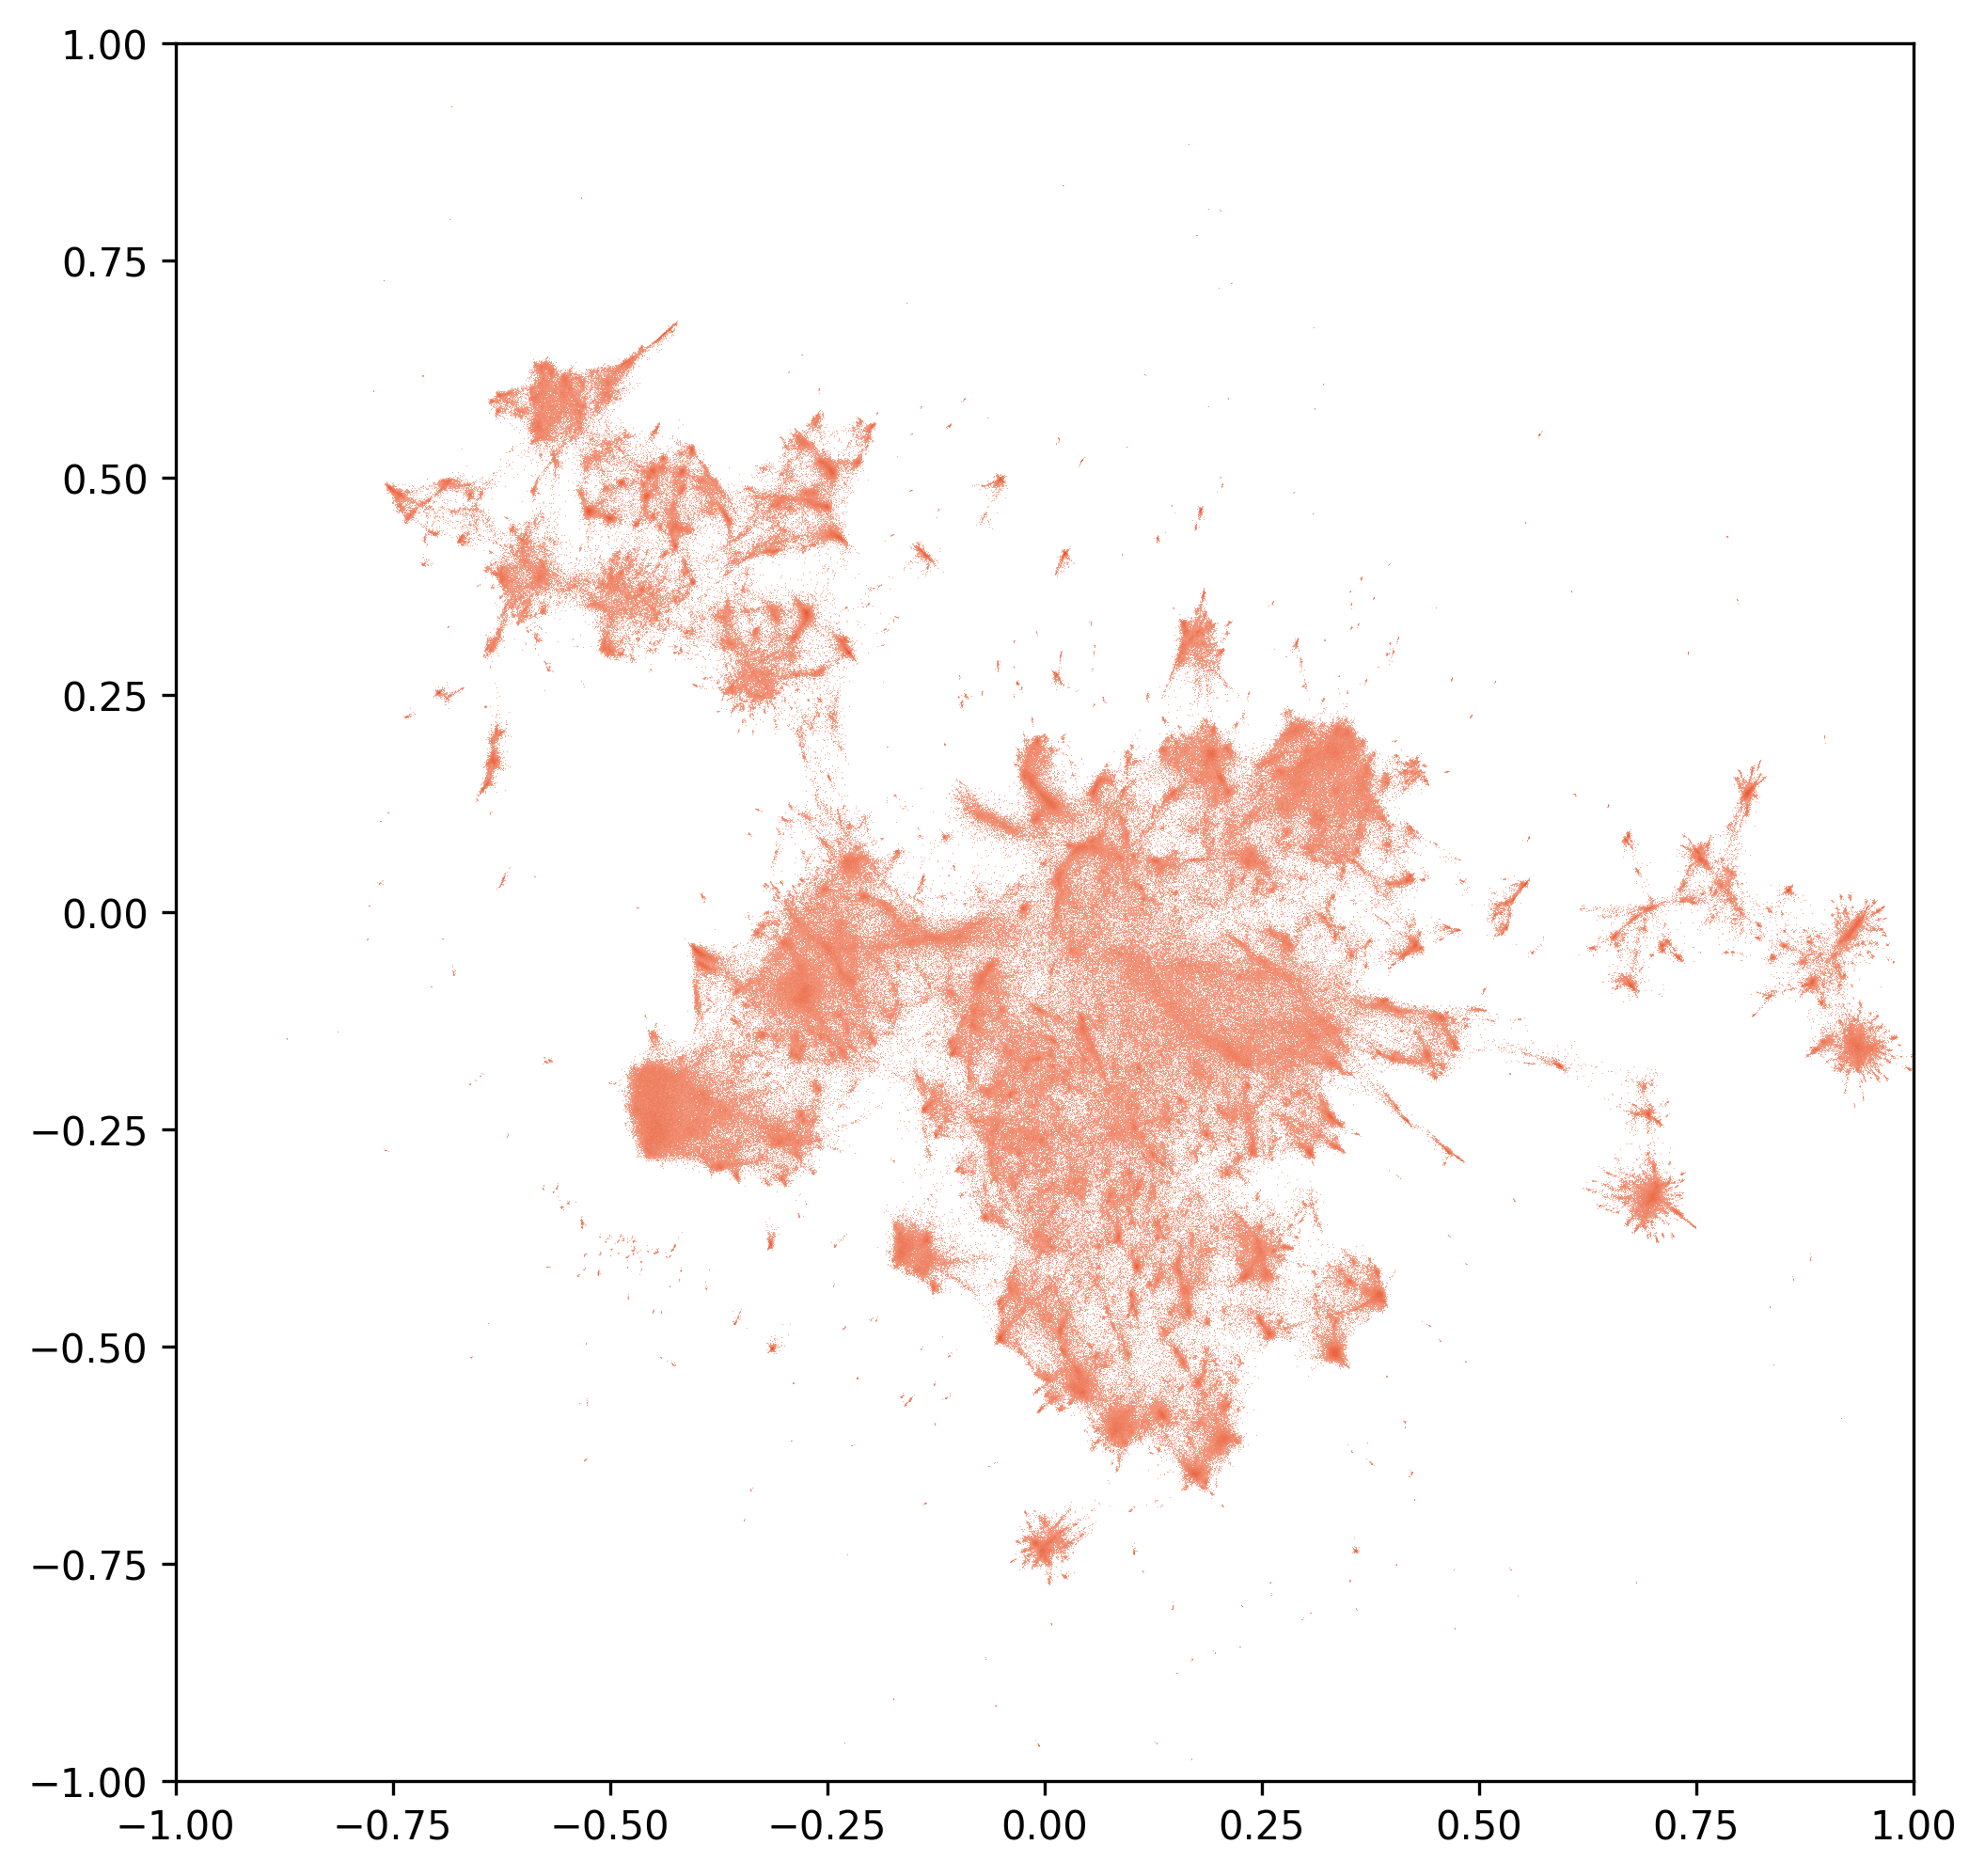
\includegraphics[width=.32\linewidth]{../src/img/all_mpnet_base_v2_umap.png}\label{fig:mpnet-umap}}
    \hfill
    \subfigure[nomic-embed UMAP]{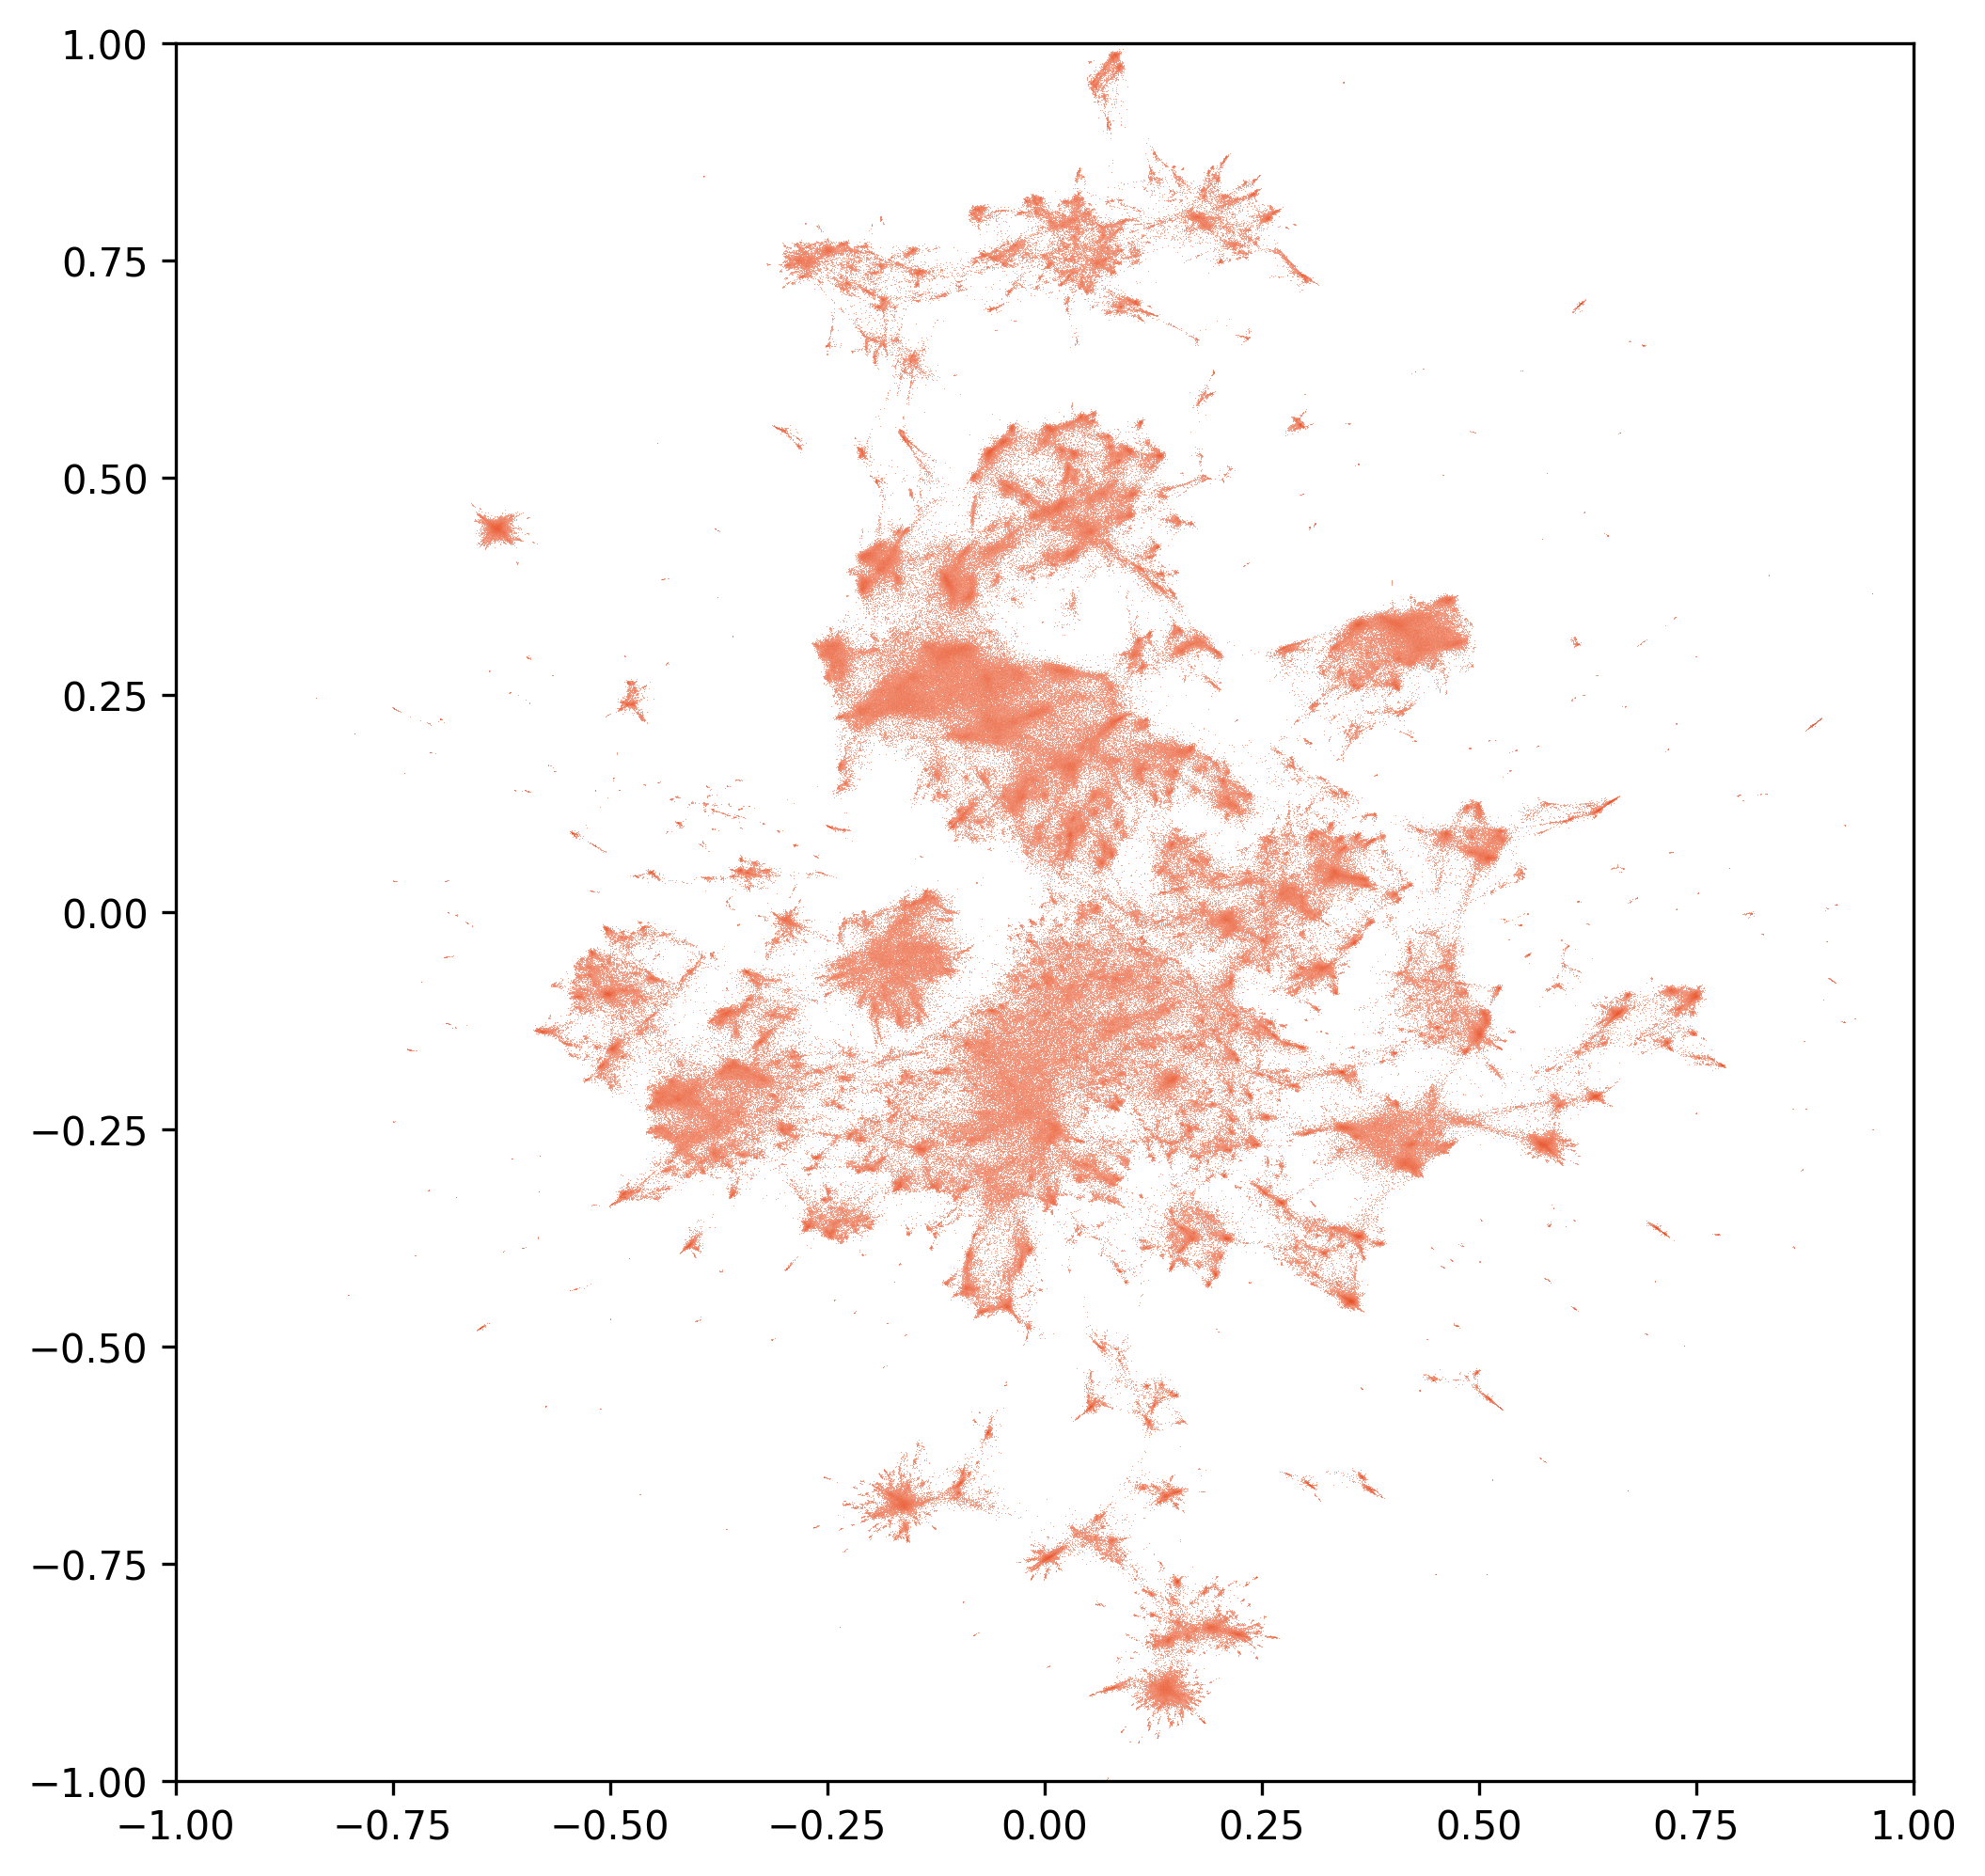
\includegraphics[width=.32\linewidth]{../src/img/nomic_embed_text_v1_5_umap.png}\label{fig:nomic-umap}}
    \caption{\label{fig:umap-series}
        Series of Uniform Manifold Approximation and Projection (UMAP) visualizations from Sentence-BERT embeddings for 1M Wikipedia articles. The projection organizes the articles by semantic similarity.}
}

\maketitle
%-------------------------------------------------------------------------
\begin{abstract}
    Continual Learning can be computationally demanding, making on-device deployment challenging. In an effort to perform dimensionality reduction that can be dynamically adjusted based on user feedback and running on-device, this paper proposes a dataset generation pipeline, providing the foundation for such a model. With a subset of the Wikipedia dataset as a source, text embeddings are generated using pretrained models such as all-MiniLM-L6-v2, all-mpnet-base-v2 and nomic-embed-text-v1.5 \cite{nussbaumNomicEmbedTraining2025}. These high-dimensional vectors are then reduced to two-dimensional coordinates by applying UMAP and t-SNE. The resulting datasets are compared and analyzed regarding their visual legibility and spatial-semantic coherence. Alongside this paper, the generation pipeline and resulting datasets are published.
\end{abstract}

%-------------------------------------------------------------------------
%-------------------------------------------------------------------------
\section{Introduction}
\label{sec:intro}

The contemporary information landscape is both vast and inflationary. This is particularly evident in technology-related fields, where professionals must constantly update, learn, and organize information to maintain effectiveness. An increasingly large portion of this cognitive effort is being supplemented with machine learning (ML): In the 2024 Stack Overflow developer survey 63.2\% of respondents reported reliance on tools that are implementing artificial intelligence \cite{AI2024Stack}.

However, the centralized architecture through which these systems are typically deployed, diminishes user ownership and autonomy. This concern extends beyond mere convenience, as recent research also suggests cognitive implications: A study by Kosmyna et al. indicates that the use of ChatGPT for essay writing is associated with decreased neural connectivity and recall ability \cite{kosmynaYourBrainChatGPT2025}.

Instead of relying on full knowledge synthesis through large language models, a more balanced approach lies in using ML to reduce the organizational overhead and friction around cognitive tasks. Addressing primarily the management and accessibility of human-generated information, this could potentially aid with comprehension and retention ability as well.

A promising strategy involves leveraging human spatial cognition. By translating the abstract, semantic relationships within a text corpus into a visual, two-dimensional plane, information can be organized in a way that is inherently intuitive. While such mappings can be generated using static dimensionality reduction (DR) techniques, a model that can continually learn and adapt the spatial layout to one's evolving needs is not yet available. The development of such a system is predicated on having a domain-specific target dataset. This paper, therefore, establishes a foundational pipeline to generate these spatial datasets from arbitrary text input. It addresses the following practical question: How can Sentence-Bert embeddings combined with Dimensionality Reduction techniques like PCA, t-SNE, and UMAP be used to generate a training dataset that maps encyclopedic texts to spatial coordinates?

The contributions are:
\begin{itemize}
    \item A concise review of relevant embedding and DR approaches (\autoref{sec:rel-work}).
    \item A reproducible pipeline as a blueprint for constructing coordinate datasets from a medium-size text corpus and pretrained encoders (\autoref{sec:main}).
    \item A brief analysis of the produced dataset configurations with regard to overall spatial structure (\autoref{sec:results}, \autoref{sec:eval} and \autoref{sec:discussion}).
\end{itemize}

%-------------------------------------------------------------------------
\section{Related Work}
\label{sec:rel-work}

Embedding generation is the prerequisite for understanding and comparing textual data. Sentence-BERT (SBERT) \cite{reimersSentenceBERTSentenceEmbeddings2019a} produces contextual embeddings that account for word order and surrounding semantics, making it a well-suited foundation in many downstream natural language processing tasks. In this work, multiple SBERT variants are used to generate these high-dimensional embedding vectors.

DR techniques such as Principal Component Analysis (PCA), t-distributed Stochastic Neighbor Embedding (t-SNE), and Uniform Manifold Approximation and Projection (UMAP) are widely applied to high-dimensional data for visualization and interactive exploration \cite{smilkovEmbeddingProjectorInteractive2016}. PCA provides a stable linear reduction and is frequently used as a preprocessing step. t-SNE remains a popular choice for uncovering fine-grained local clusters but is computationally demanding. The OpenTSNE implementation improves efficiency and scalability, making it more suitable for medium to large datasets \cite{policarOpenTSNEModularPython2024}. UMAP, in contrast, emphasizes global structure while still preserving local neighborhoods \cite{mcinnesUMAPUniformManifold2020a}.

Finally, commercial systems such as Nomic Atlas \cite{duderstadtAtlasWhitepaperScalable} adopt a similar approach, embedding large-scale corpora and projecting them into low-dimensional interactive maps. Atlas is designed for scalability and integrates with projection frameworks such as NOMAD \cite{nussbaumNomicEmbedTraining2025}. However, parts of the system remain proprietary, limiting reproducibility. In contrast, the dataset generation pipeline proposed here is aimed at small models suitable for continual learning while remaining fully open-source.

%-------------------------------------------------------------------------
\section{Dataset Generation from Dimensionality Reduction}
\label{sec:main}

The pipeline is implemented as a two-stage process designed to represent semantic similarity as spatial proximity. Initially, the source text corpus is converted into high-dimensional semantic embeddings, which are then subsequently reduced to two-dimensional coordinates.

%-------------------------------------------------------------------------
\subsection{Pipeline Implementation}
\label{subsec:pipeline}

The pipeline's implementation prioritizes modularity and reproducibility. Its components are fully exchangeable via standard Hugging Face APIs, a design choice that allows for the flexible testing of various models and parameters for domain-specific applications. To ensure consistent and reproducible results, the random seed for all non-deterministic processes is fixed to $97$. As a practical demonstration, this paper utilizes the Wikipedia dataset \cite{WikimediaWikipediaDatasets2025} (\texttt{20231101.en} configuration) as its source corpus. To manage computational demands within hardware and scope constraints, development and testing were performed on a subset of $n=1M$ articles. The complete pipeline is illustrated in \autoref{fig:pipeline-overview}. The workstation specifications are as follows:

\begin{itemize}
    \item An Intel Core i9-10980XE (3.00GHz) CPU
    \item An NVIDIA Quadro RTX 5000 (16GB) GPU
    \item 128 GB of RAM
\end{itemize}

\begin{figure*}[!htb]
    \centering
    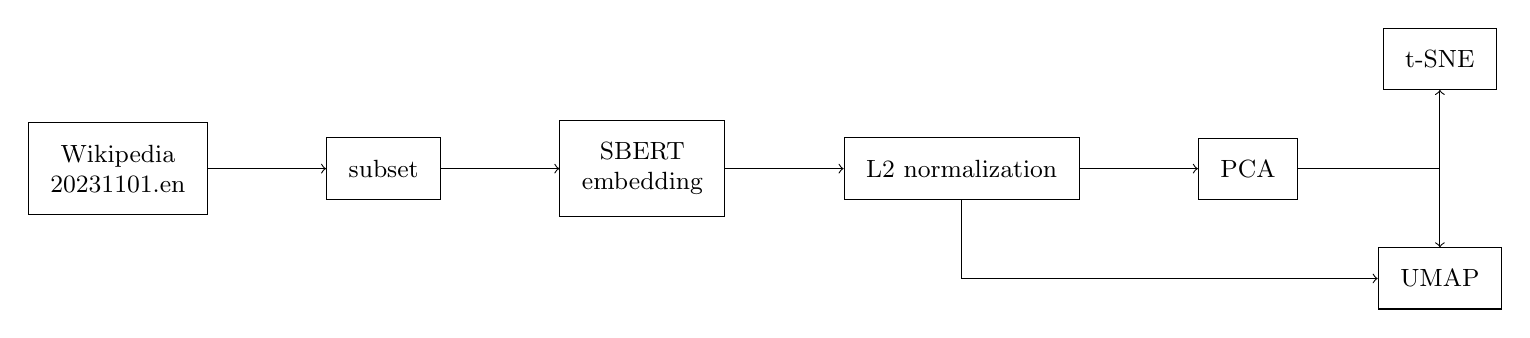
\begin{tikzpicture}[
            scale=0.9,
            node distance=1cm and 1.5cm,
            box/.style={draw, rectangle, align=center, font=\small, inner sep=0.28cm}
        ]
        \node[box] (A) {Wikipedia\\20231101.en};
        \node[box, right=of A] (B) {subset};
        \node[box, right=of B] (C) {SBERT\\embedding};
        \node[box, right=of C] (D) {L2 normalization};
        \node[box, right=of D] (F) {PCA};

        \coordinate (split) at ($(F.east)+(2,0)$);

        \node[box, above=of split] (G) {t-SNE};
        \node[box, below=of split] (H) {UMAP};

        \draw[->] (A) -- (B);
        \draw[->] (B) -- (C);
        \draw[->] (C) -- (D);
        \draw[->] (D) -- (F);
        \draw[->] (D) |- (H);

        \draw[->] (F.east) -- (split) -| (G.south);
        \draw[->] (F.east) -- (split) -| (H.north);
    \end{tikzpicture}
    \caption{Schematic overview of the dataset generation pipeline components: A subset of 1M entries is selected from the Wikipedia dataset. Each SBERT model is used to generate an embedding. The results are normalized to Euclidean space (L2 normalization). PCA with a reduction to 50 dimensions is applied before the final dimensionality reduction step using t-SNE. The UMAP is computed both with and without the prior PCA preprocessing.}
    \label{fig:pipeline-overview}
\end{figure*}

\subsubsection{Embedding Generation Stage}
\label{sec:embed-gen}

The pipeline employs three distinct pre-trained sentence transformer models for text embedding generation:

\begin{enumerate}
    \item \texttt{all-MiniLM-L6-v2}: A lightweight model based on the MiniLM architecture, optimized for efficiency while maintaining competitive performance on semantic similarity tasks.
    \item \texttt{all-mpnet-base-v2}: A model utilizing the MPNet (Masked and Permuted Pre-training) architecture, which combines the advantages of BERT and XLNet through bidirectional attention and permutation-based training.
    \item \texttt{nomic-embed-text-v1.5}: A specialized embedding model with extended context length capabilities, specifically designed for clustering applications and requiring task-specific prompting \cite{nussbaumNomicEmbedTraining2025}.
\end{enumerate}

For the smaller models (1. and 2.), text inputs are processed without additional prompting. Due to their limited context windows, texts exceeding the maximum token length are truncated during tokenization, potentially resulting in information loss for longer texts. The larger model (3.) is configured with a clustering-specific prompt ("clustering: ") to optimize embedding quality for the downstream DR step. Its larger context size enables processing of complete articles without truncation, preserving the full semantic content of the inputs. Batch processing is implemented with model-specific batch sizes: $32$ samples for the two smaller models and $16$ samples for 3., balancing computational efficiency with memory constraints.

\subsubsection{Preprocessing Stage}
\label{sec:preprocessing}

Prior to dimensionality reduction, embeddings undergo a preprocessing procedure:

All embedding vectors are L2-normalized to unit length, transforming the similarity metric from cosine similarity to Euclidean distance. This normalization ensures that subsequent distance-based algorithms operate in a geometrically consistent space.

As a common strategy to accelerate t-SNE, a PCA transformation to 50 dimensions is performed. This is an increase from the 30 dimensions used in the original implementation by van der Maaten and Hinton \cite{JMLR:v9:vandermaaten08a}, made feasible by improvements in the openTSNE library \cite{policarOpenTSNEModularPython2024} for datasets of this scale. Besides performance gains, this step also aids in noise reduction \cite{JMLR:v9:vandermaaten08a}. Therefore, UMAP is applied to both the PCA-preprocessed embeddings and the original vectors to evaluate the impact of this preprocessing step (see \autoref{fig:tsne-umap-comparison} bottom row (d-f) for comparison).

\subsubsection{Dimensionality Reduction Stage}

The final stage of the pipeline reduces the high-dimensional embeddings into a two-dimensional space using the aforementioned two complementary non-linear techniques: UMAP and t-SNE.

The \texttt{umap-learn} library \cite{mcinnesUMAPUniformManifold2020a} is utilized to generate two distinct configurations. The first is applied directly to the full-dimensional, L2-normalized embeddings using the default "spectral" initialization. The second is applied to the 50-dimensional data resulting from the PCA preprocessing step. For this second variant, the UMAP algorithm is initialized using an additional PCA reduction to the target dimension. This strategy provides a more informed starting point for the internal optimization process, which can accelerate convergence.

In contrast, the more computationally demanding t-SNE reduction is performed exclusively on the lower dimensional PCA processed data. The \texttt{openTSNE} implementation is further optimized by leveraging parallel processing. Analogous to UMAP, PCA is used as an initialization strategy here as well. It is important to note that only default hyperparameters were used for both algorithms. This choice was made intentionally, as the pipeline is presented as an adaptable blueprint for domain-specific applications where subsequent fine-tuning would be a necessary step.

Following the reduction, a final normalization step is applied to all generated coordinates. Using the MinMaxScaler from the \texttt{scikit-learn} \cite{pedregosaScikitlearnMachineLearning2018} library, the 2D coordinates for each output are scaled to a consistent range of $\left[-1,1\right]$. This ensures that the outputs from different models and configurations inhabit a uniform geometric space, facilitating direct visual and quantitative comparison. To provide a comprehensive performance analysis, runtimes for each individual step of the pipeline were measured. The total execution time was also recorded (excluding the initial dataset loading phase).

%-------------------------------------------------------------------------
\subsection{Result}
\label{sec:results}

\begin{table}[h!]
    \centering
    \pgfplotstabletypeset[
        col sep=comma,
        columns={dataset,step,time},
        columns/dataset/.style={column name=\textbf{Dataset}, column type=|l|, string type, verb string type},
        columns/step/.style={column name=\textbf{Step}, column type=l|, string type, verb string type},
        columns/time/.style={column name=\textbf{Time}, column type=l|, fixed, fixed zerofill, precision=2},
        every head row/.style={before row=\hline, after row=\hline},
        every last row/.style={after row=\hline},
    ]{../src/eval/pipeline-runtimes-1000000-20251013_075621.csv}
    \caption{Runtimes for the pipeline components measured in seconds. The total runtime was measured across the full execution (excluding dataset loading times)}
    \label{tab:runtimes}
\end{table}

\begin{figure*}[htb]
    \centering
    \subfigure[all-MiniLM-L6-v2 t-SNE]{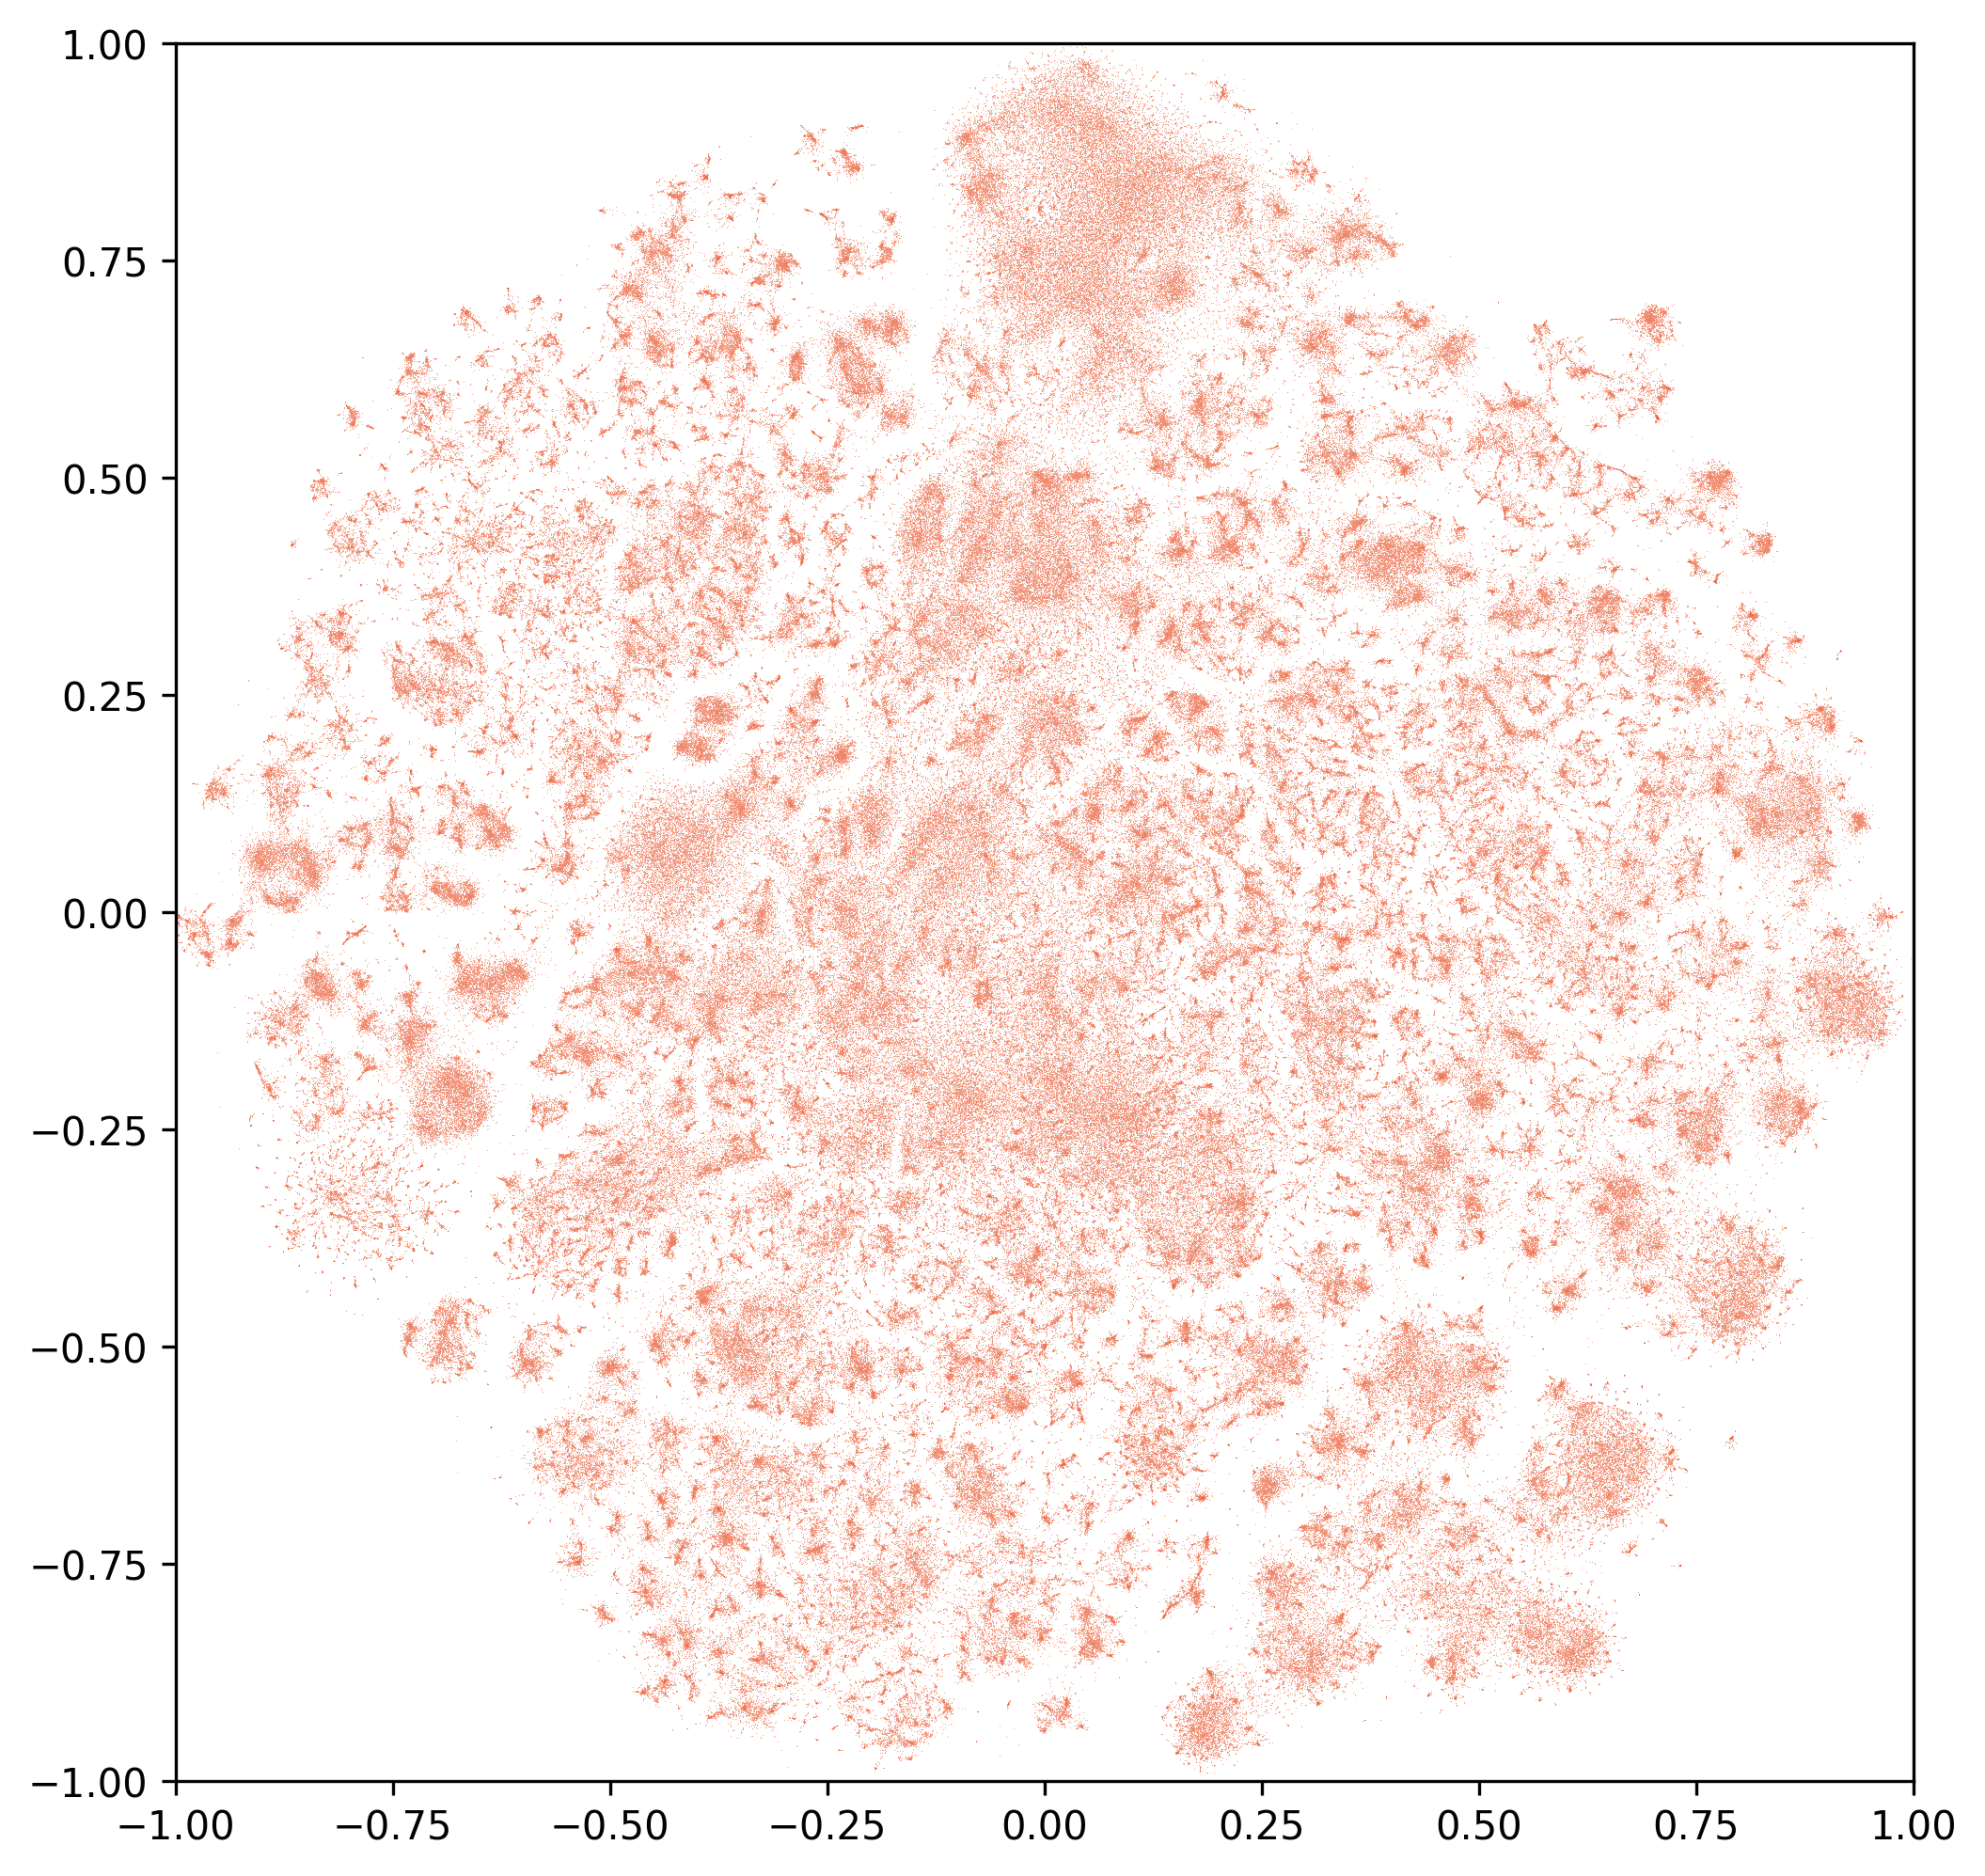
\includegraphics[width=.32\linewidth]{../src/img/all_MiniLM_L6_v2_tsne.png}\label{fig:minilm-tsne}}
    \hfill
    \subfigure[all-mpnet-base-v2 t-SNE]{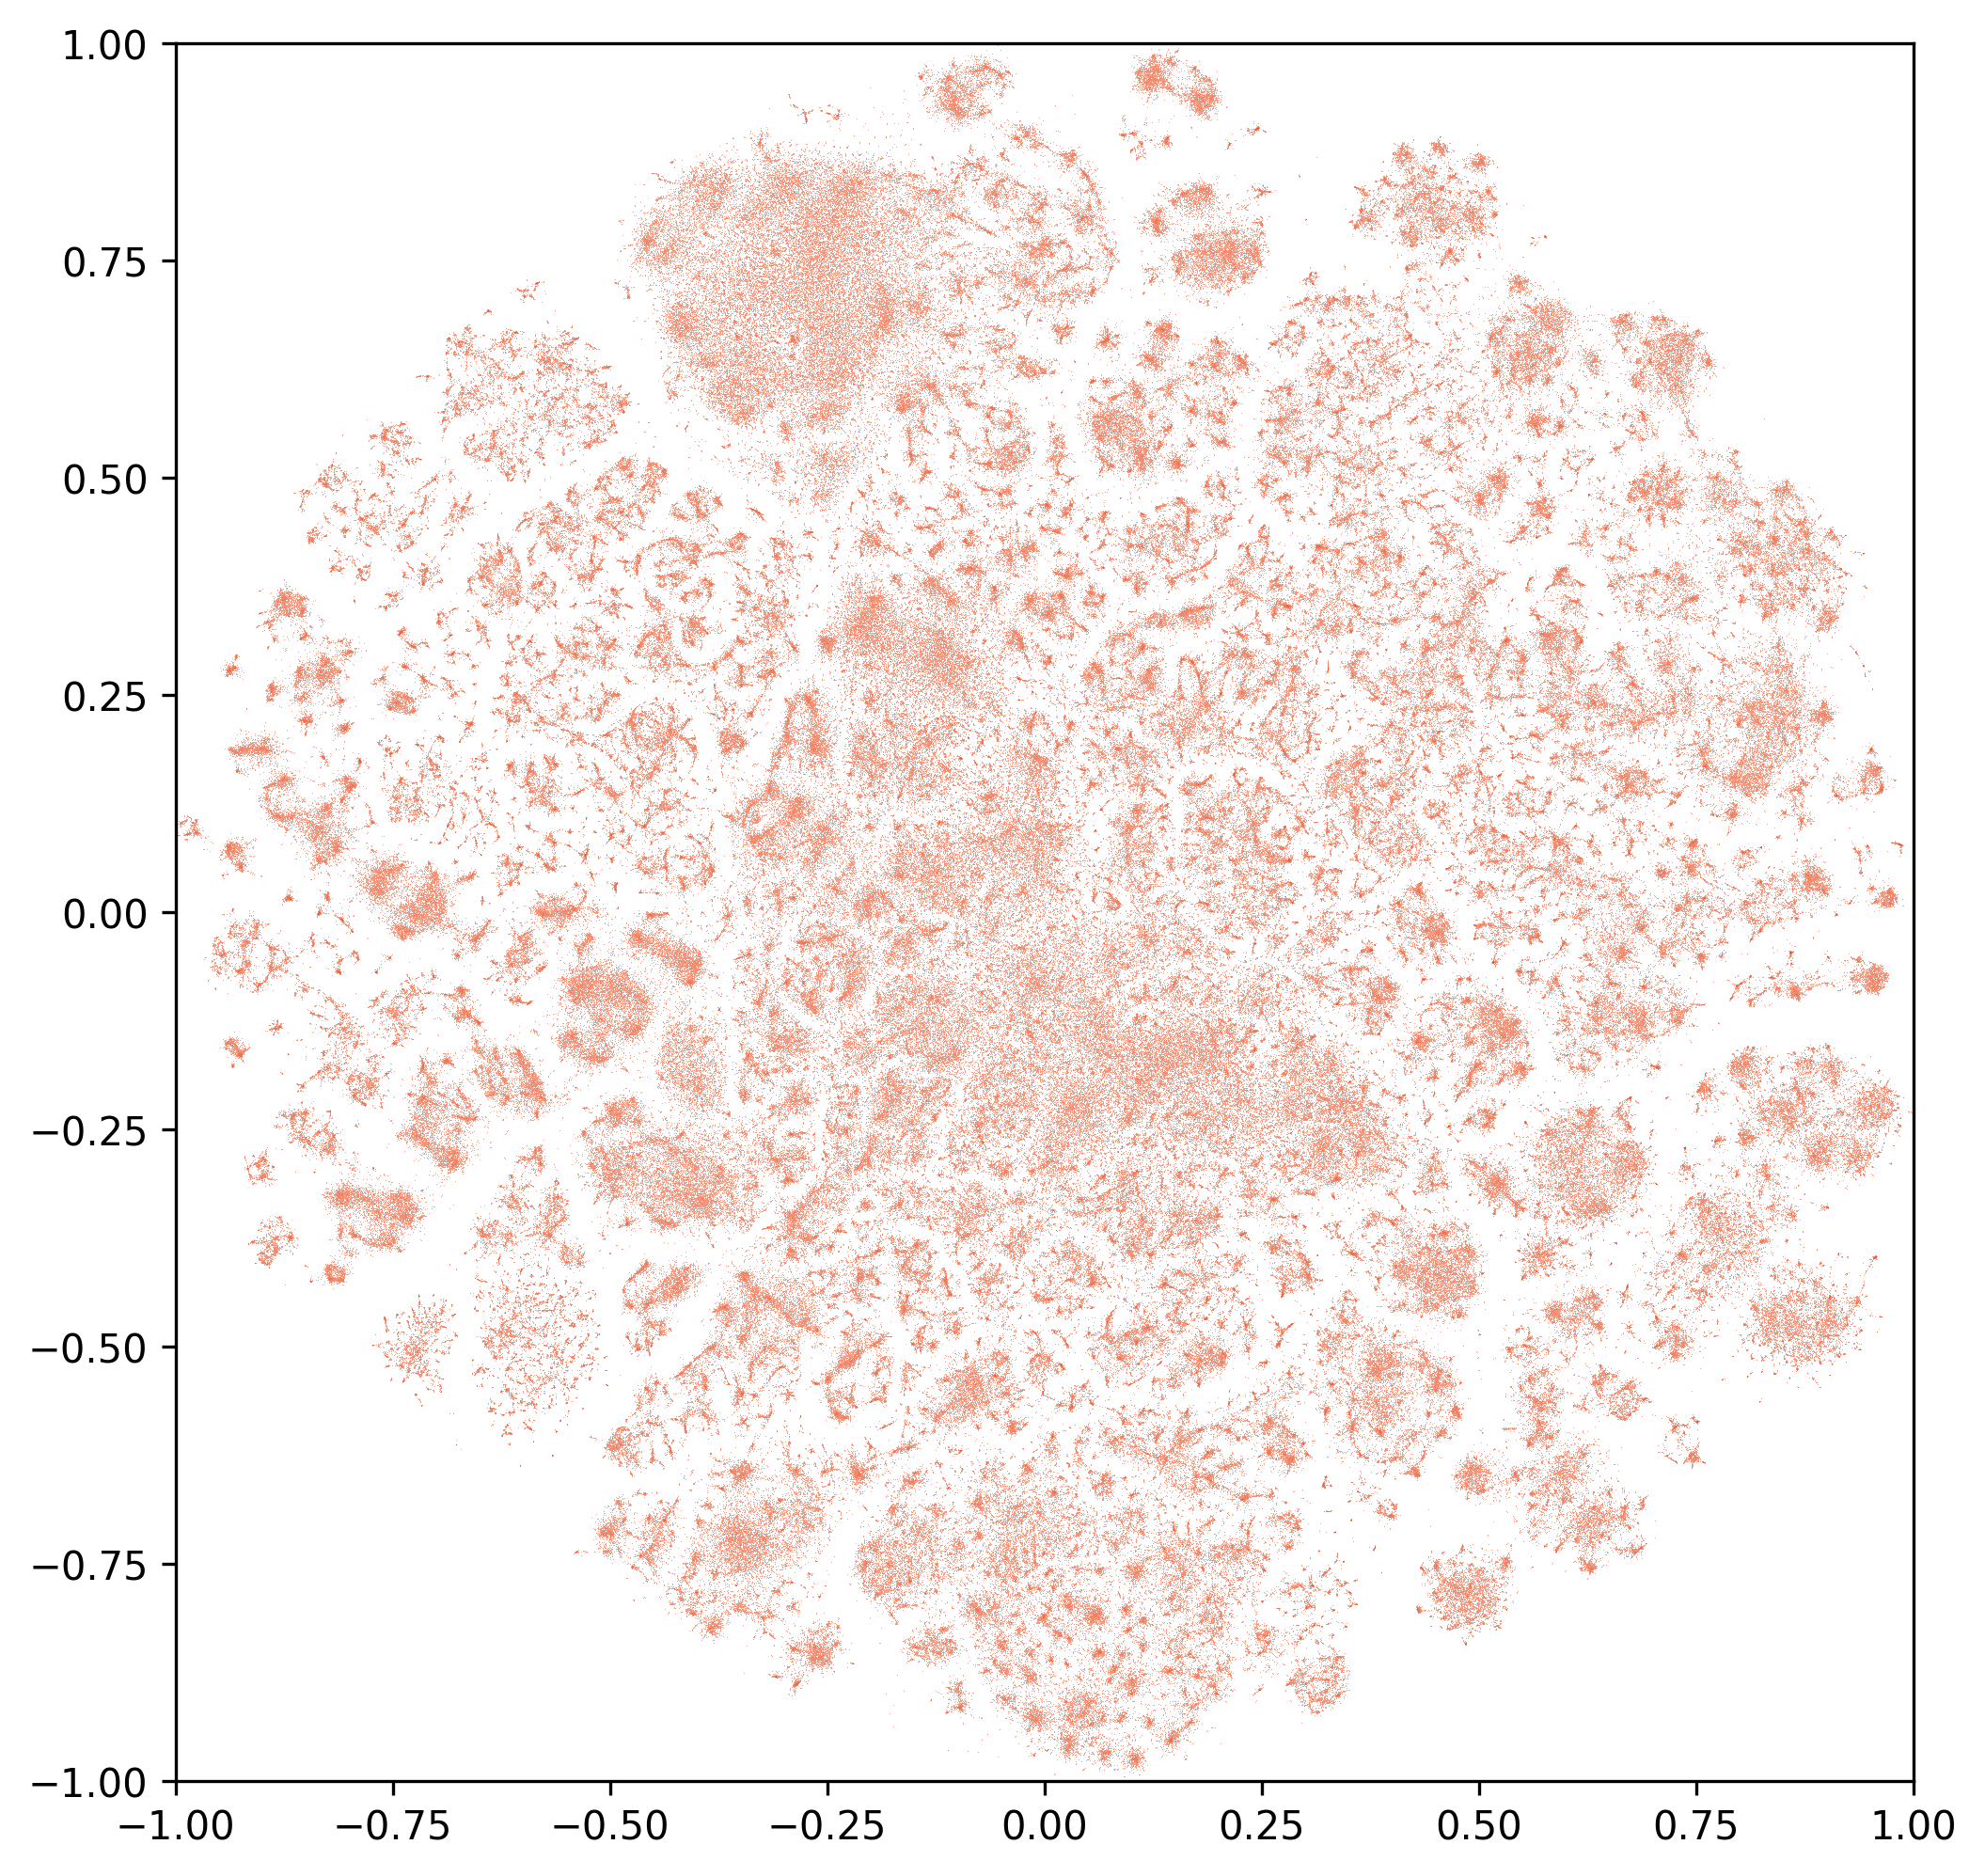
\includegraphics[width=.32\linewidth]{../src/img/all_mpnet_base_v2_tsne.png}\label{fig:mpnet-tsne}}
    \hfill
    \subfigure[nomic-embed t-SNE]{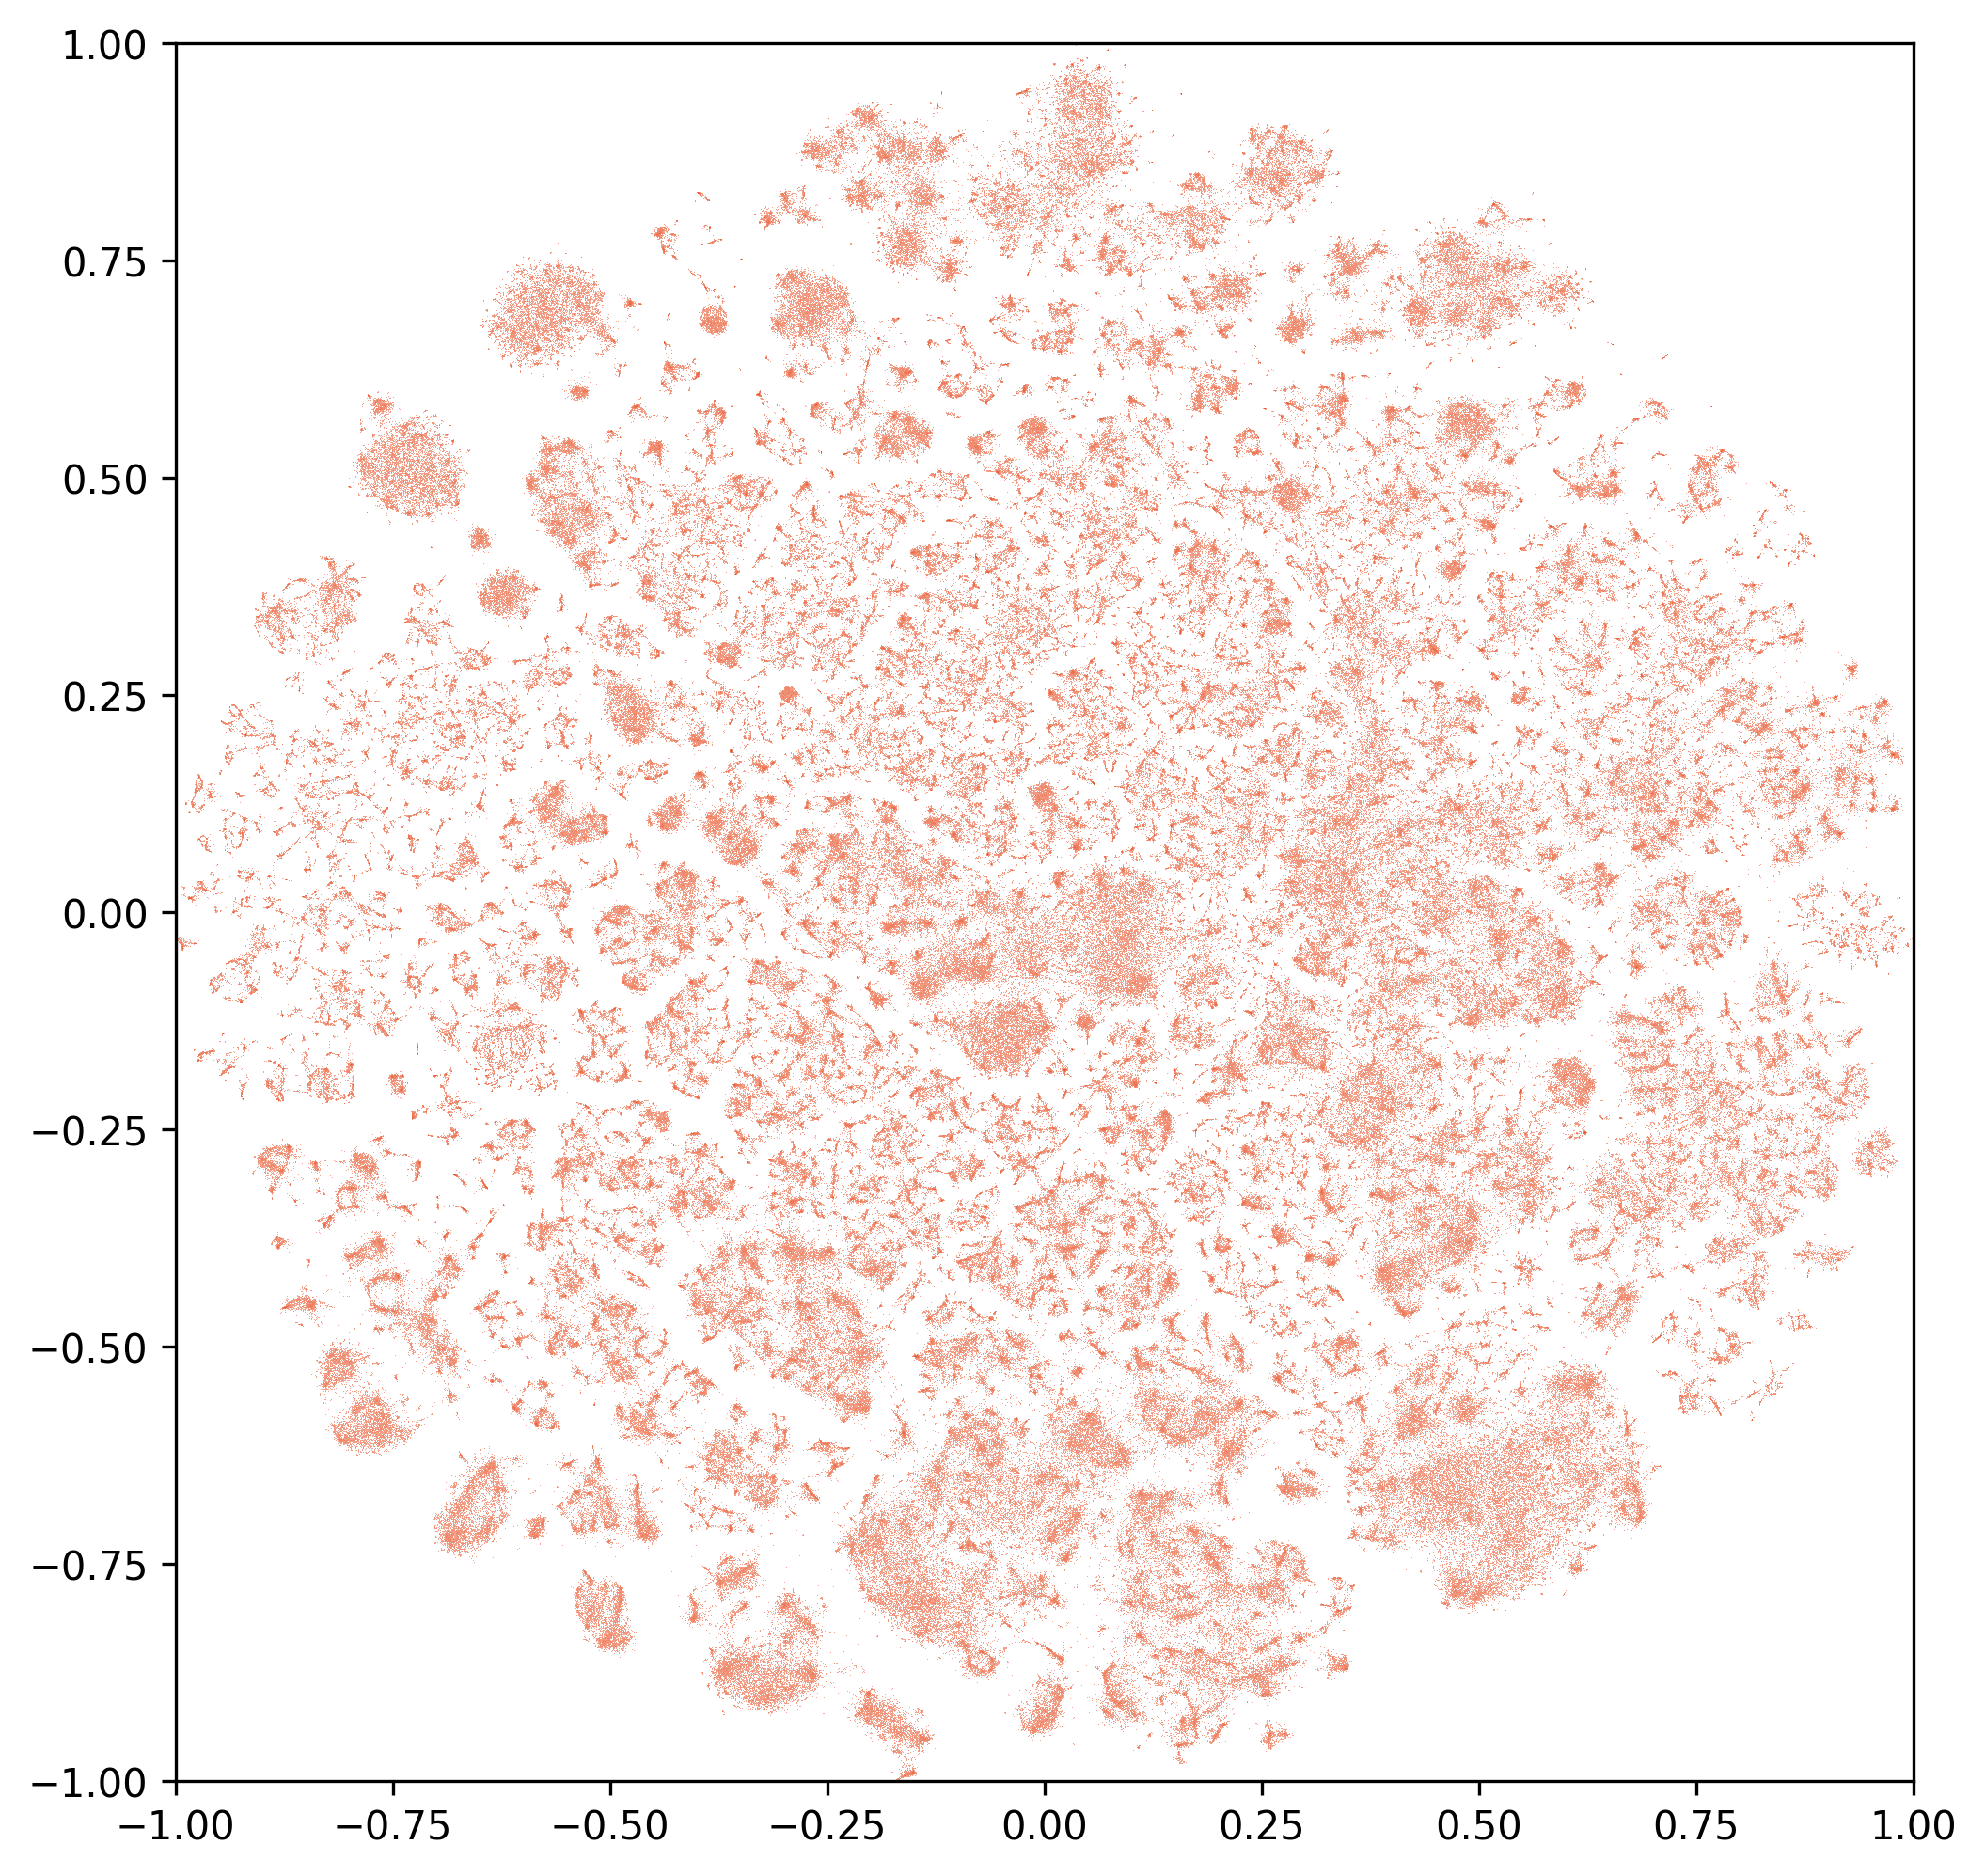
\includegraphics[width=.32\linewidth]{../src/img/nomic_embed_text_v1_5_tsne.png}\label{fig:nomic-tsne}}
    \\[1em]
    \subfigure[all-MiniLM-L6-v2 PCA UMAP]{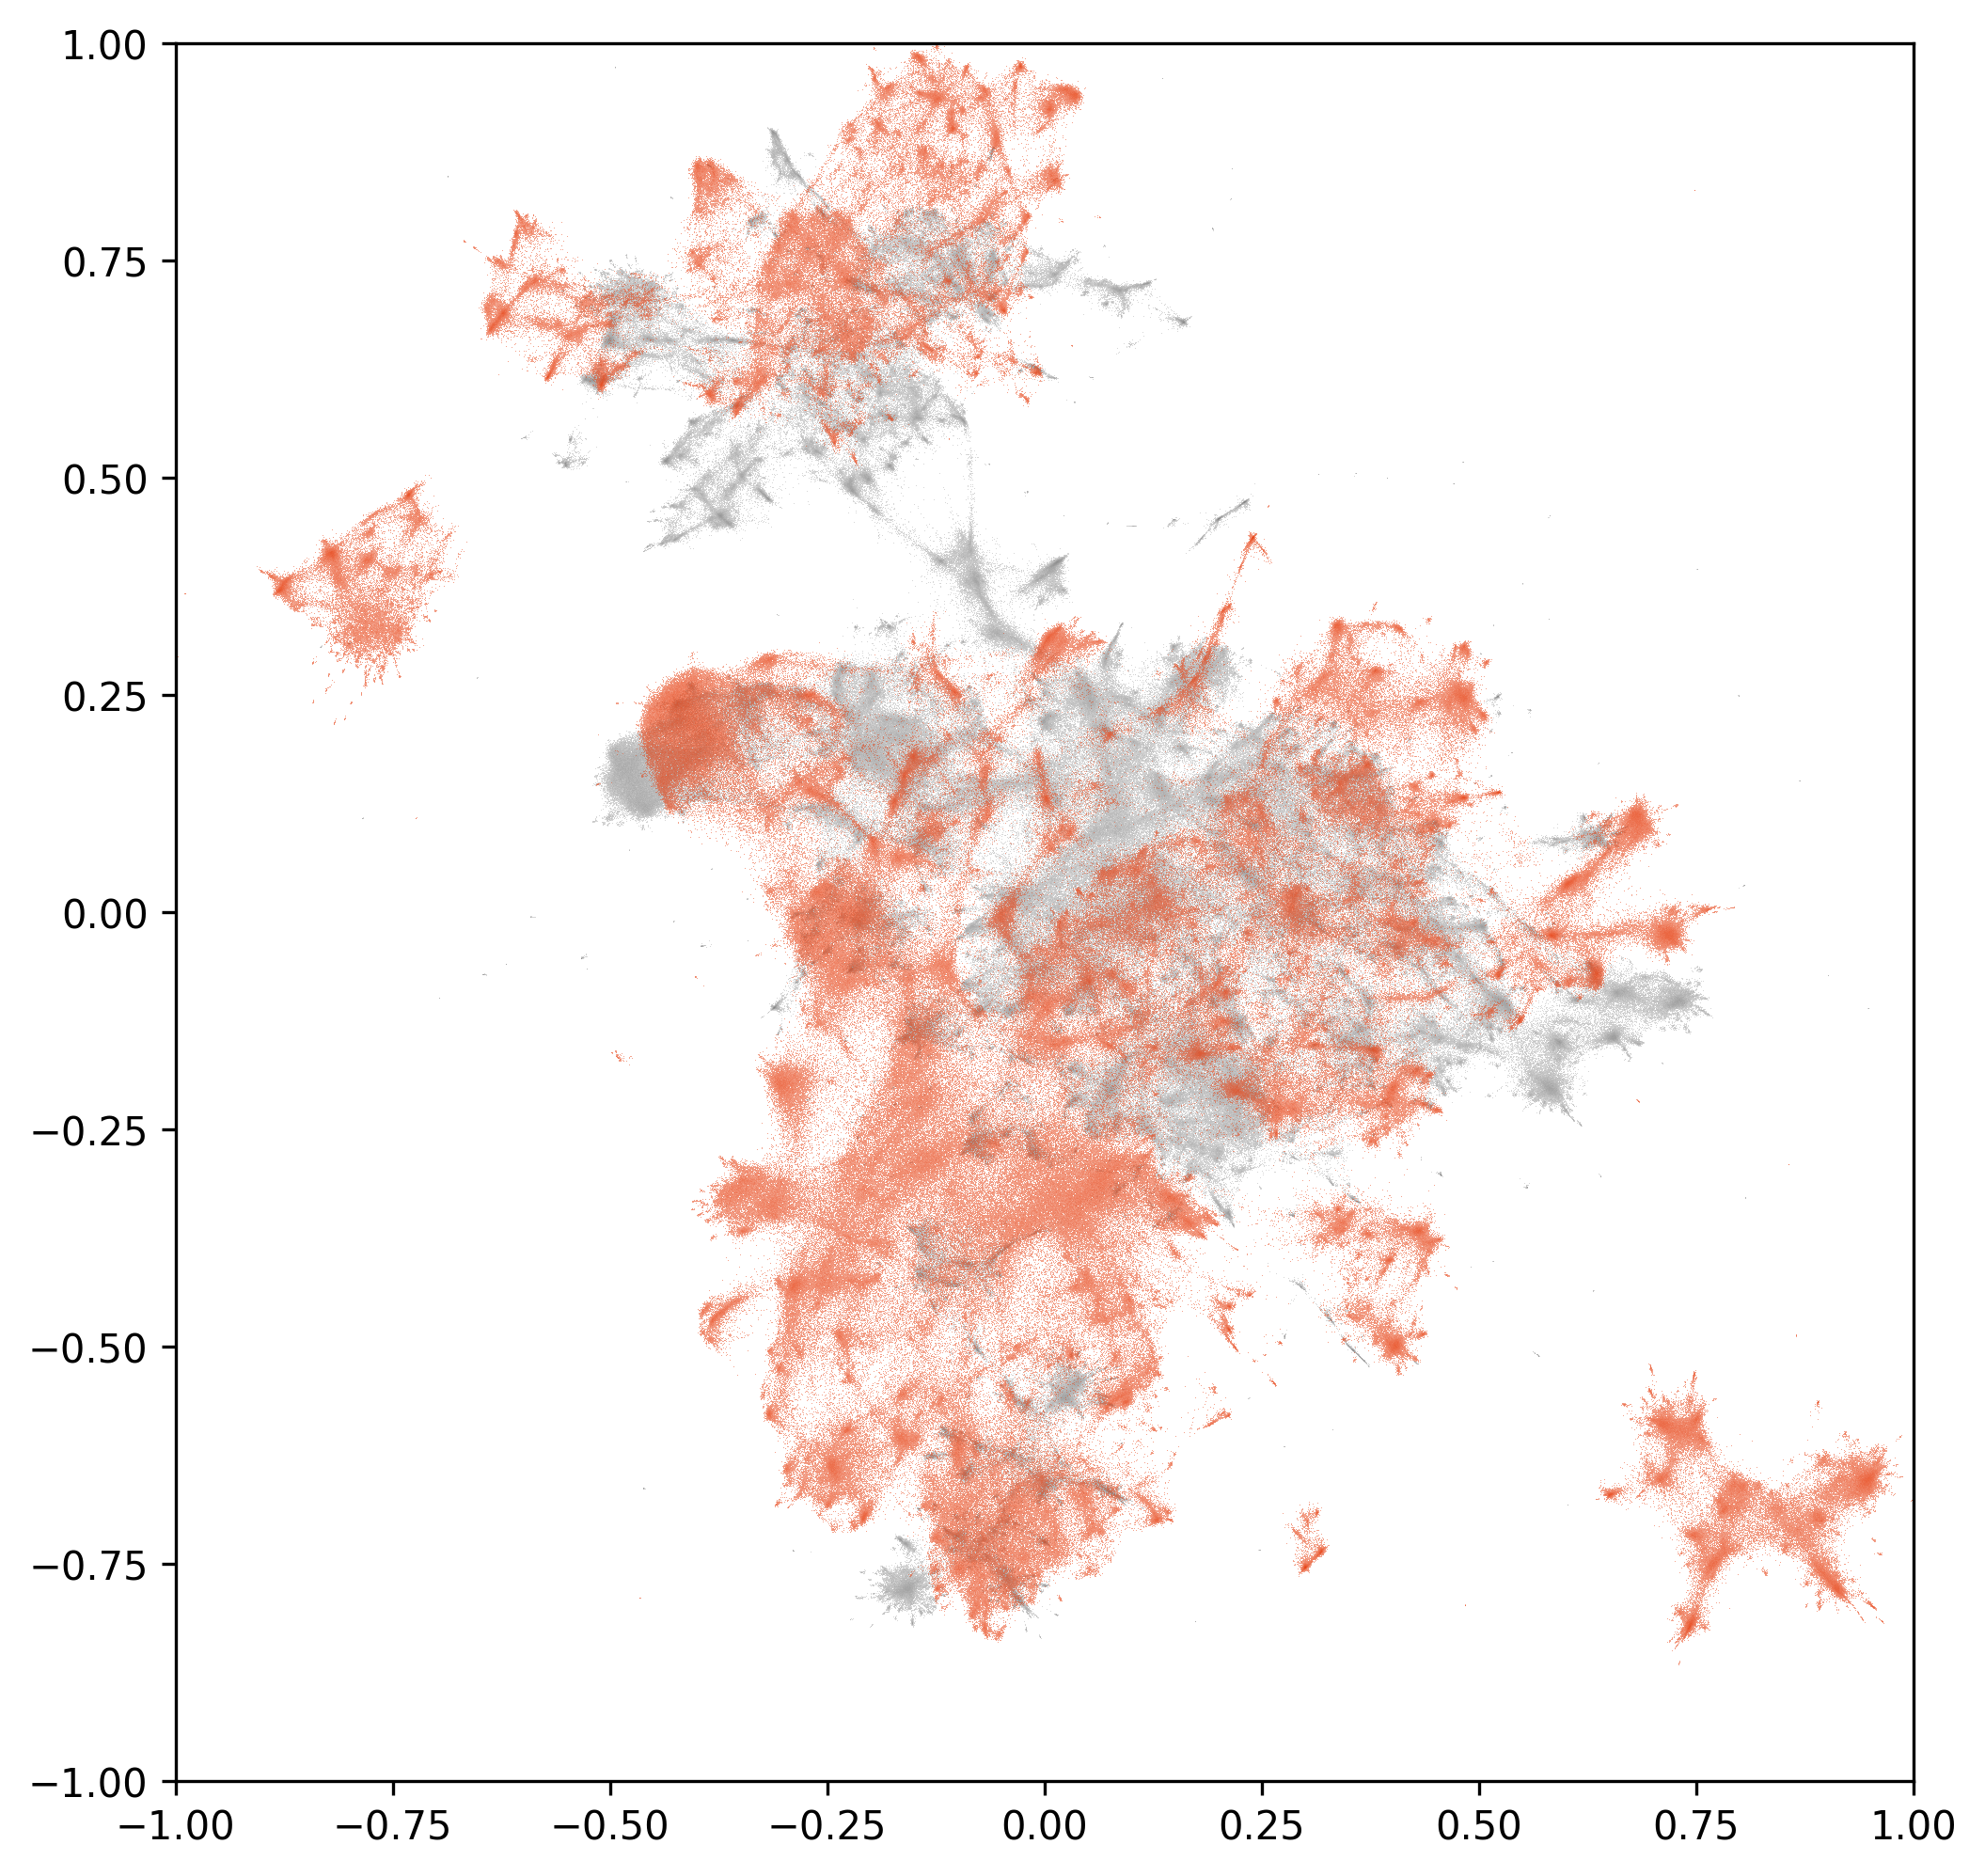
\includegraphics[width=.32\linewidth]{../src/img/all_MiniLM_L6_v2_umap_pca.png}\label{fig:minilm-umap-pca}}
    \hfill
    \subfigure[all-mpnet-base-v2 PCA UMAP]{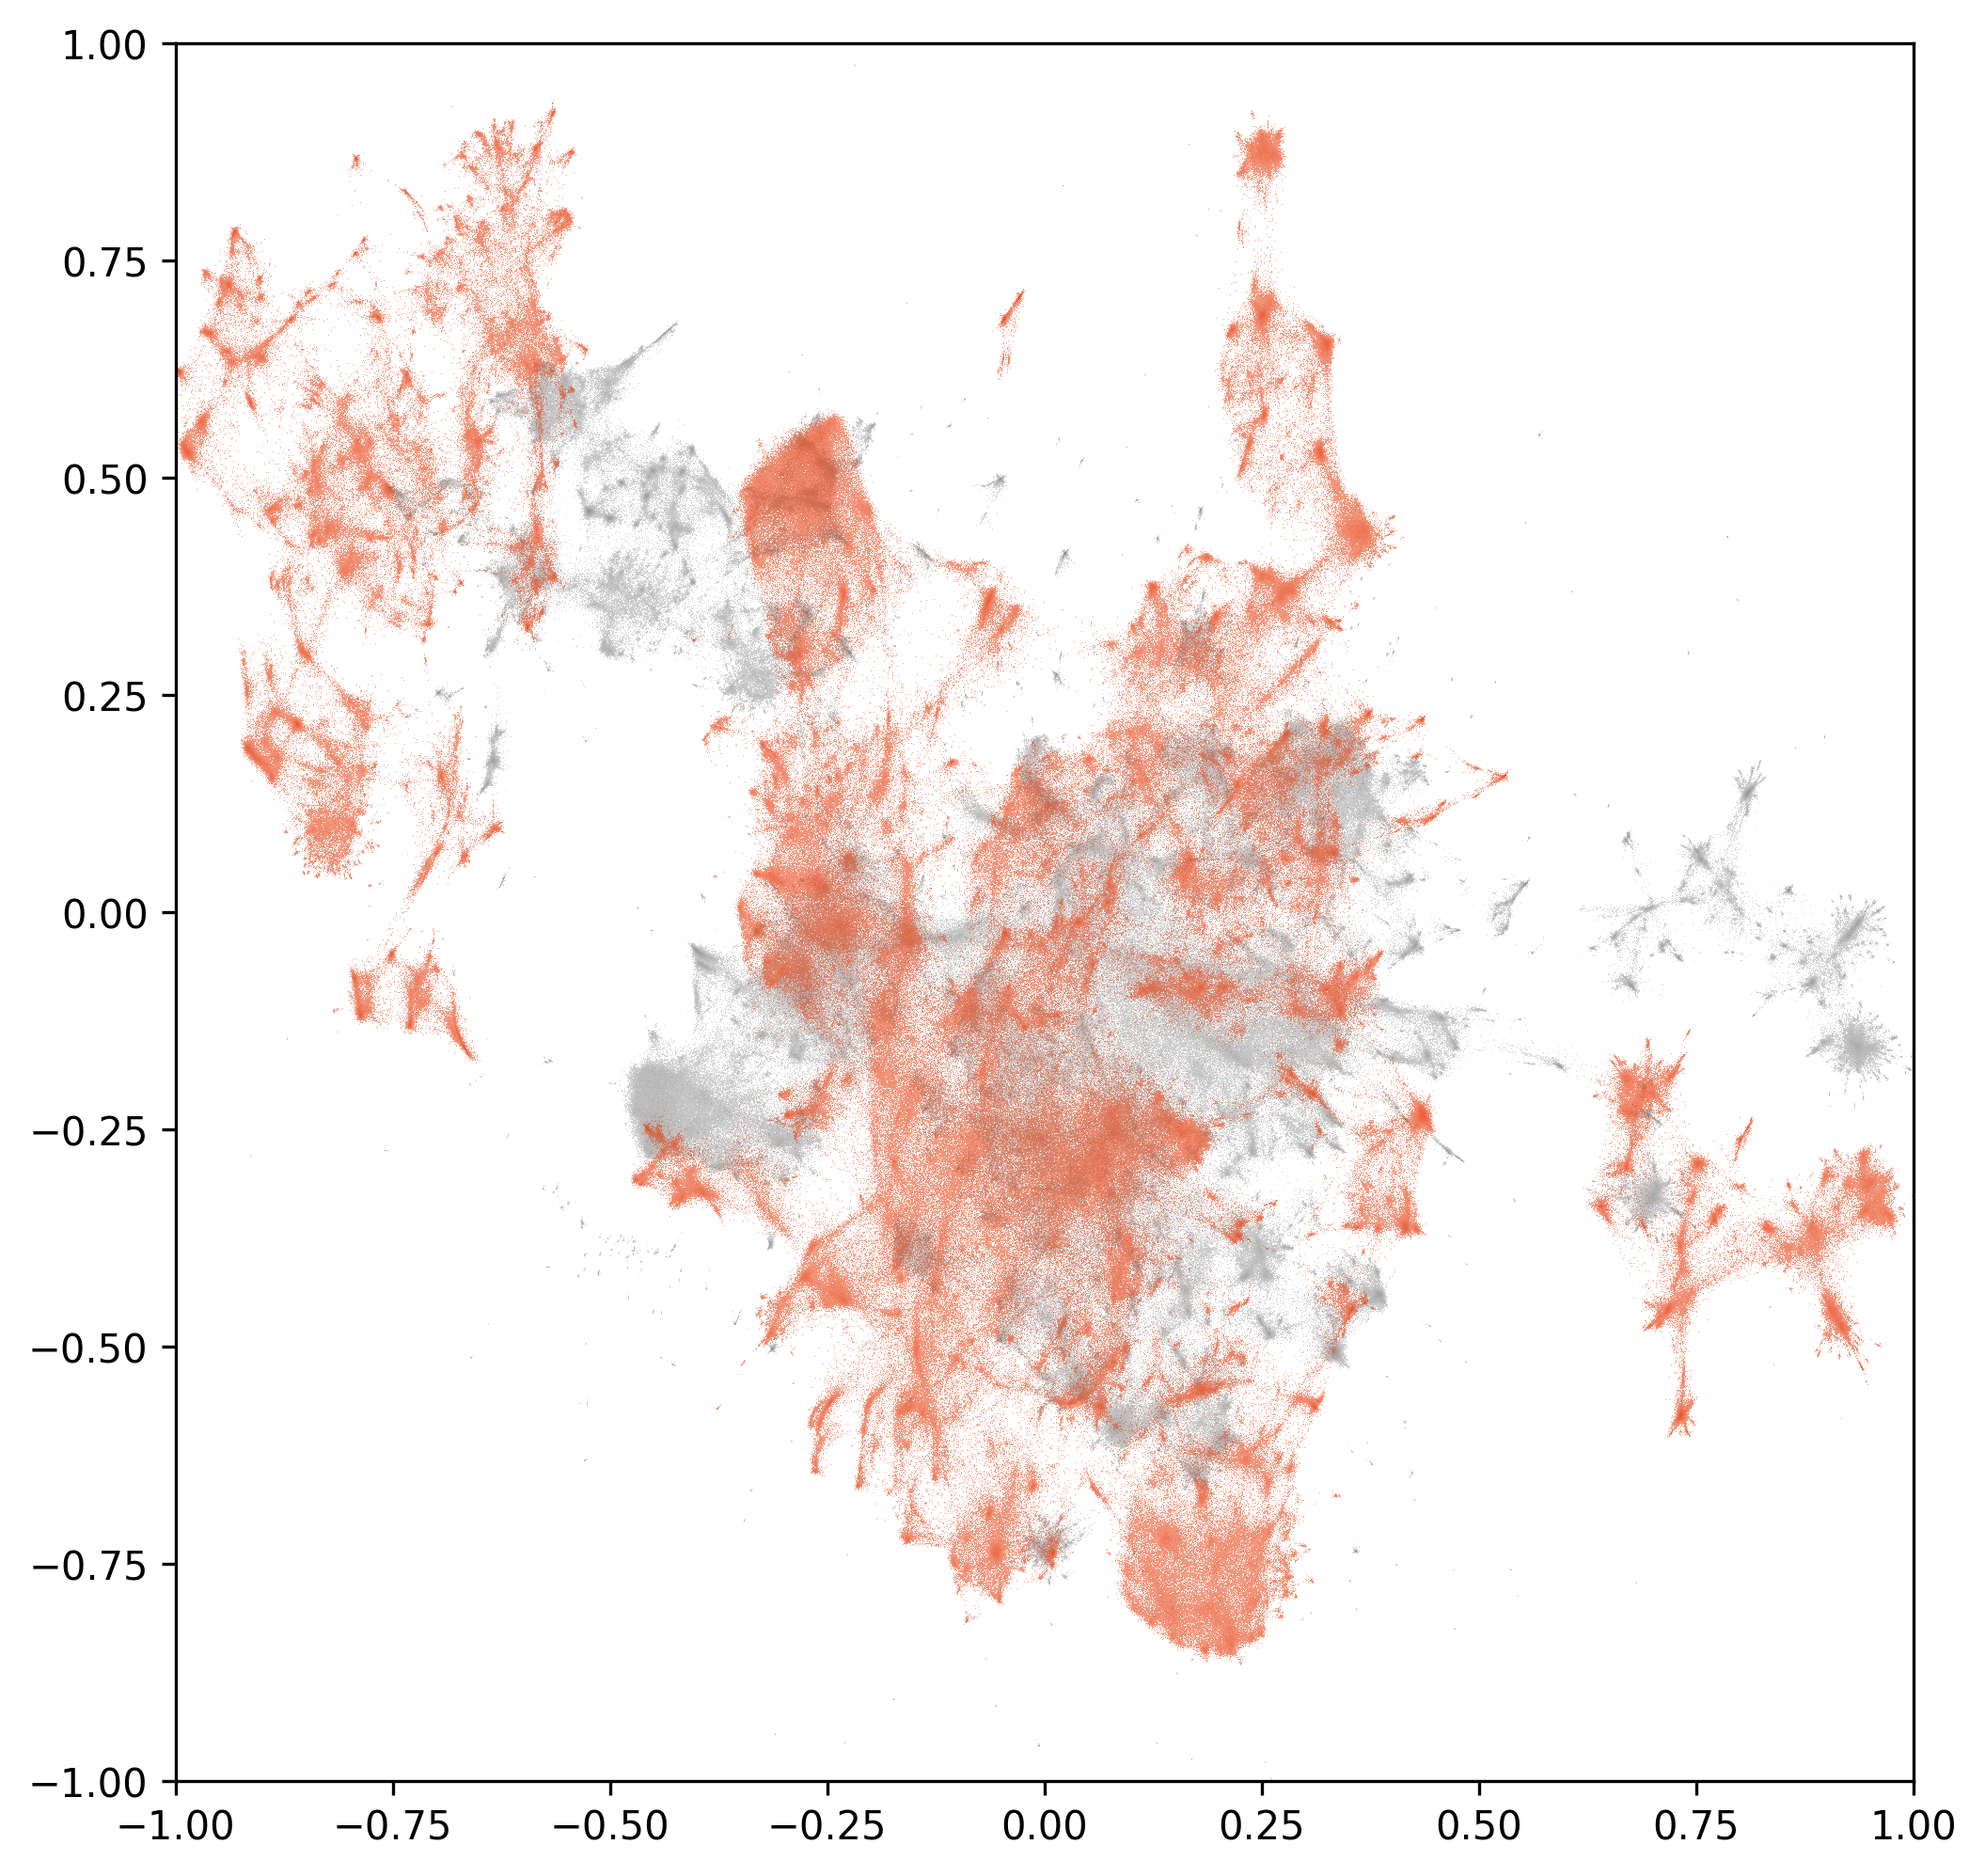
\includegraphics[width=.32\linewidth]{../src/img/all_mpnet_base_v2_umap_pca.png}\label{fig:mpnet-umap-pca}}
    \hfill
    \subfigure[nomic-embed PCA UMAP]{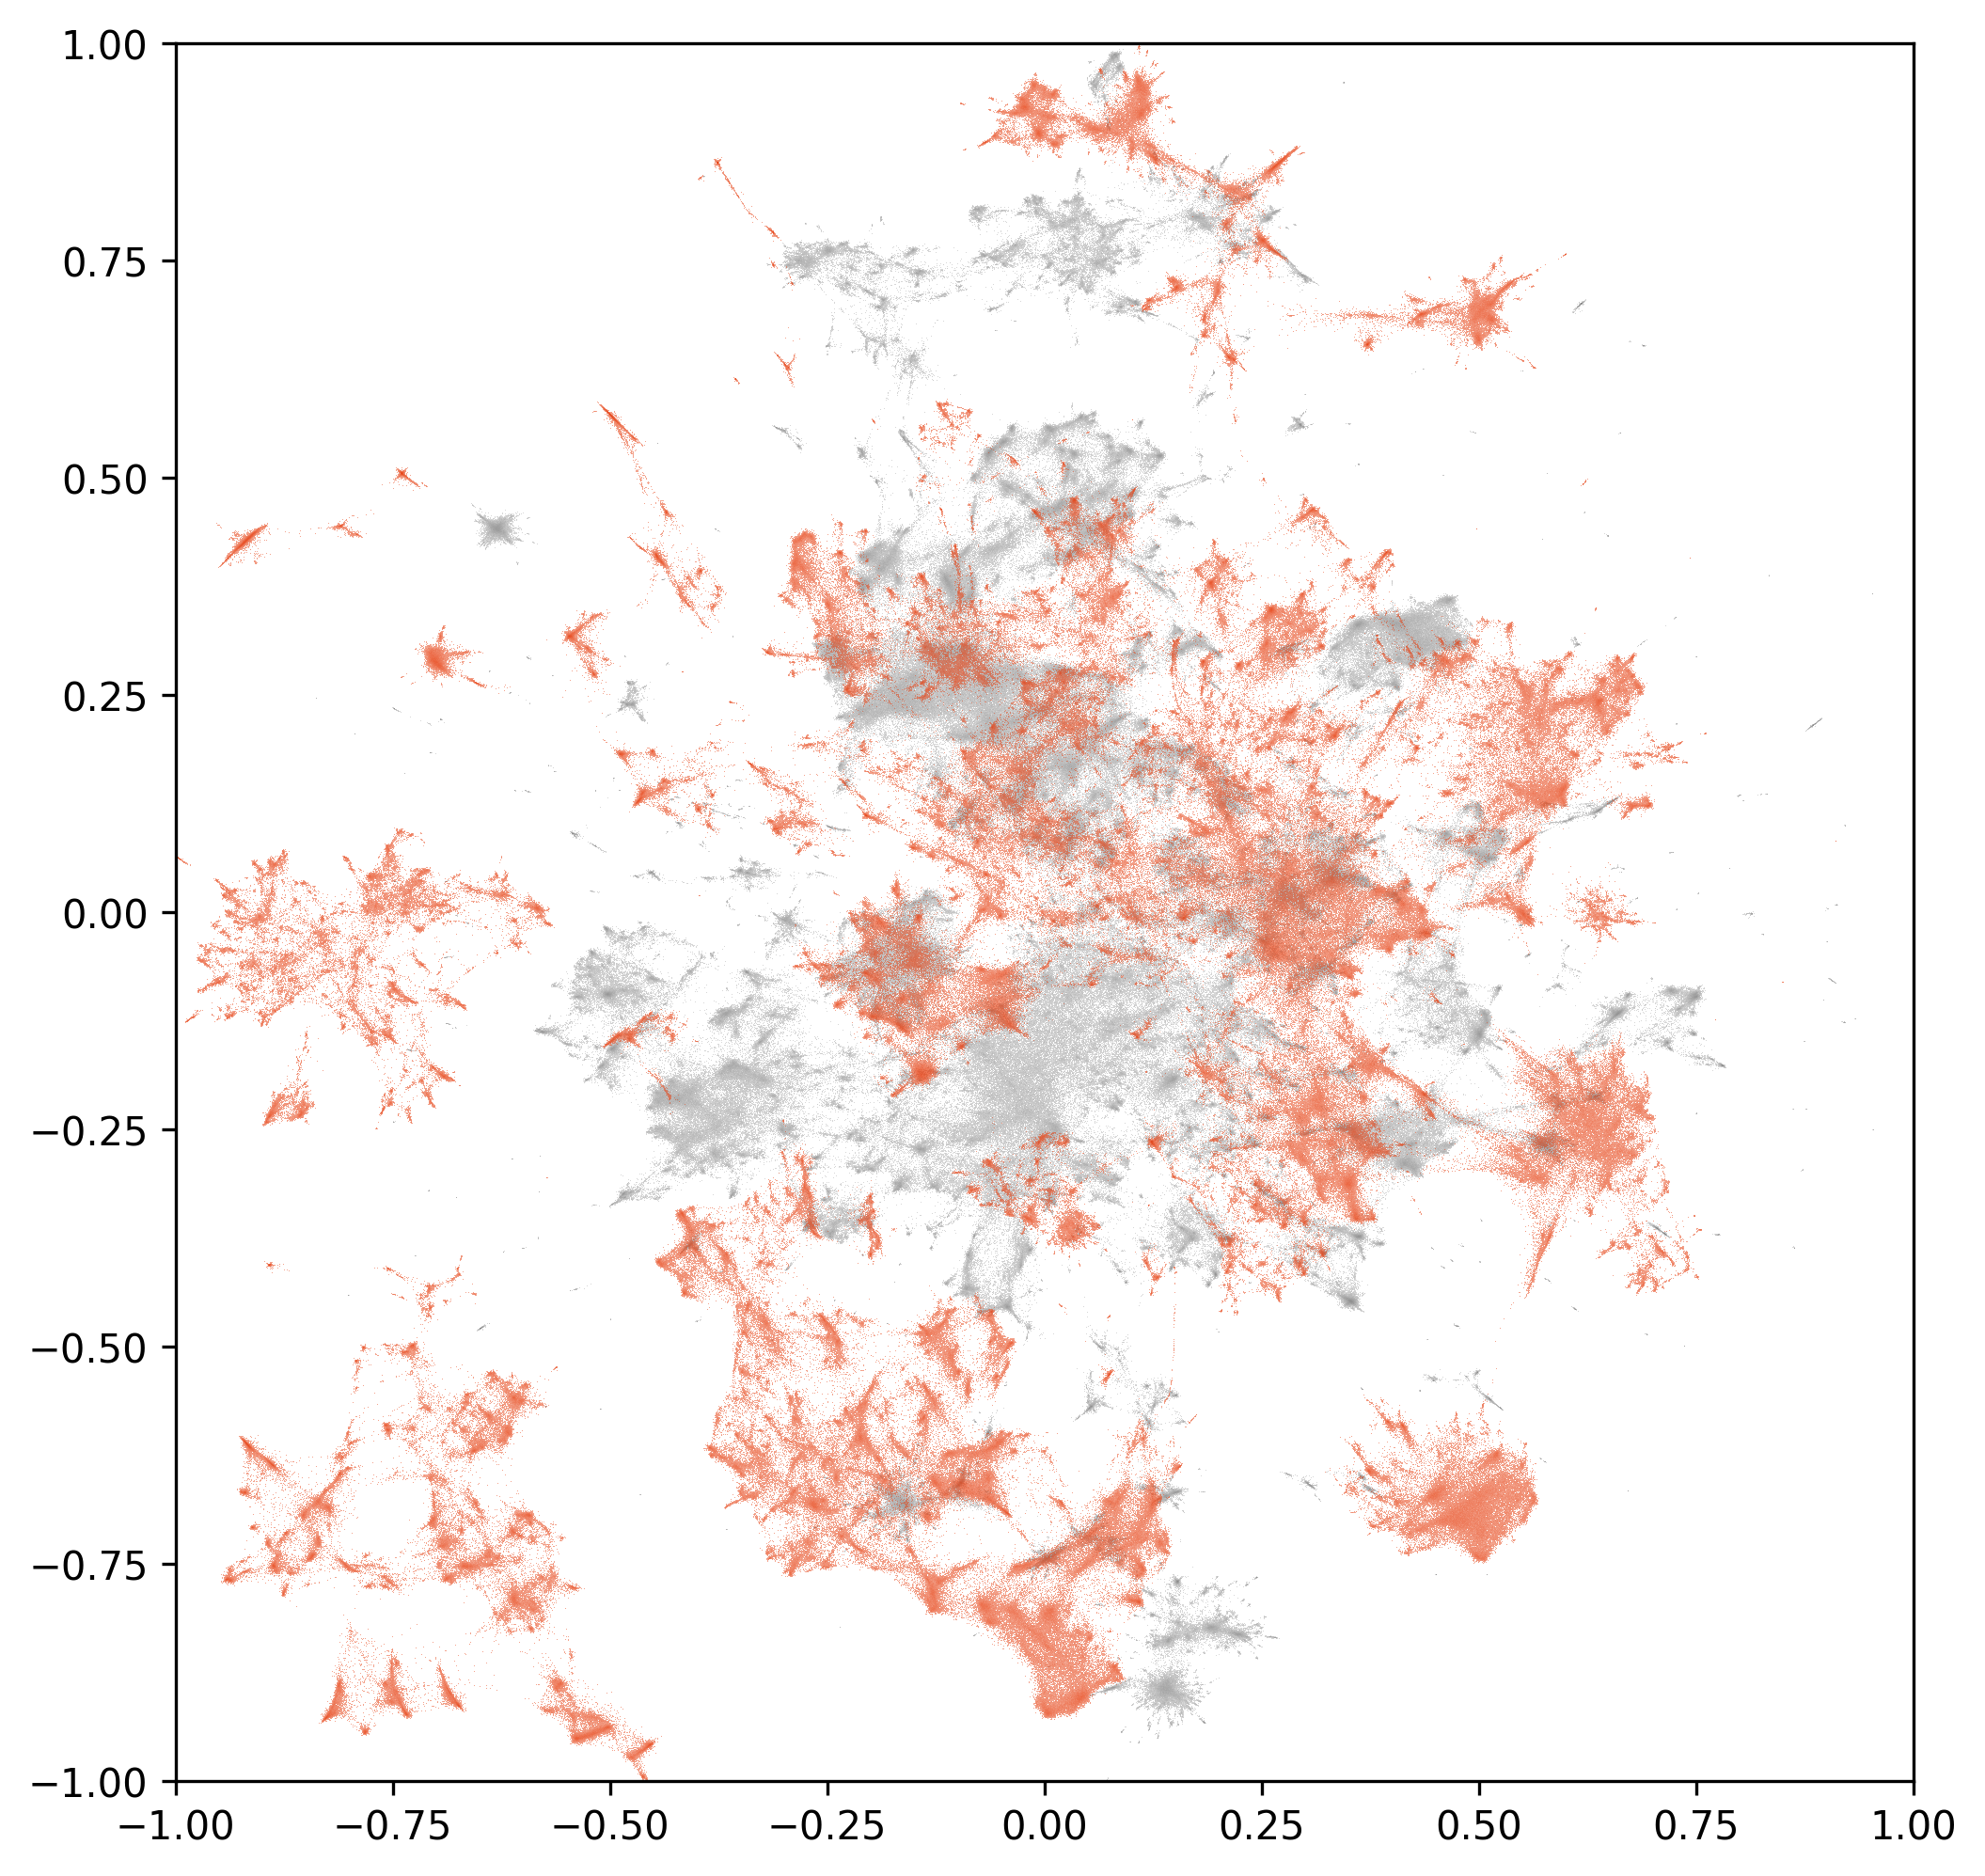
\includegraphics[width=.32\linewidth]{../src/img/nomic_embed_text_v1_5_umap_pca.png}\label{fig:nomic-umap-pca}}
    \caption{Series of reduced and normalized SBERT embeddings. The top row (a-c) is comprised of t-SNE embeddings, preprocessed with PCA. The Bottom row (d-f) displays a comparison of both UMAP configurations: Direct reduction of the full-length SBERT embedding (grey coordinates) as seen in \autoref{fig:umap-series} and the PCA preprocessed projection (orange coordinates).}
    \label{fig:tsne-umap-comparison}
\end{figure*}

The pipeline successfully processed the text corpus, transforming the high-dimensional embeddings into a series of two-dimensional coordinate datasets. The resulting spatial arrangements, visualized in \autoref{fig:umap-series} and \autoref{fig:tsne-umap-comparison}, reveal distinct structural characteristics depending on the chosen embedding model and reduction configuration. These projections exhibit a range of topologies, from landscape-like formations with pronounced global structures to more evenly distributed clusters that emphasize local neighborhoods. Each visualization provides a unique representation of the corpus's underlying semantic organization.

On the specified hardware a full execution cycle was completed in under a full day (about 21.74 hours). The embedding generation was the primary bottleneck with the \texttt{nomic-embed-text-v1-5} variant responsible for over half of the total runtime (about 13.22 hours). Detailed runtimes for each component individually are presented in \autoref{tab:runtimes}.

%-------------------------------------------------------------------------
\subsection{Evaluation}
\label{sec:eval}

Evaluating the output of unsupervised dimensionality reduction (DR) presents a significant challenge, as there are no explicit labels to measure against. The core problem shifts from measuring accuracy to quantifying the trustworthiness of the low-dimensional representation. To address this, the quantitative approach described by Kury et al. \cite{kuryDREAMSPreservingBoth2025} was adopted, assessing the quality of the projection by measuring the preservation of local and global structures from the original high-dimensional embedding space. The two key metrics used are:

\begin{itemize}
    \item \textbf{k-Nearest Neighbor Recall (KNN)}: It operates by checking, for each data point, what proportion of its original nearest neighbors in the high-dimensional space are still its nearest neighbors in the final 2D projection. A higher KNN score indicates that the immediate, fine-grained relationships between data points have been successfully maintained.
    \item \textbf{Correlation of Pairwise Distances (CPD)}: This metric evaluates the preservation of the global structure by calculating the Spearman's rank correlation between the distances of point pairs. It compares the distances between a random sample of data points in the original high-dimensional space to their corresponding distances in the low-dimensional map. A strong positive correlation signifies that the overall layout and large-scale topology of the data have been faithfully represented.
\end{itemize}

The implementation in this paper is based on similar methods proposed by Kobak and Berens \cite{kobakArtUsingTSNE2019}. Both scoring algorithms were implemented with the same parameters the authors used ($k=10$ for KNN and CPD on $1000$ randomly chosen entries).

\begin{table}[h!]
    \centering
    \pgfplotstabletypeset[
        col sep=comma,
        columns={config,knn,cpd},
        columns/config/.style={column name=\textbf{Configuration}, column type=|l|, string type, verb string type},
        columns/knn/.style={column name=\textbf{KNN}, column type=c|, fixed, fixed zerofill, precision=4},
        columns/cpd/.style={column name=\textbf{CPD}, column type=c|, fixed, fixed zerofill, precision=4},
        every head row/.style={before row=\hline, after row=\hline},
        every last row/.style={after row=\hline},
    ]{../src/eval/eval-None-20251012_031840.csv}
    \caption{Evaluation results showing k-nearest neighbor recall (KNN) and correlation of pairwise distances (CPD) scores as described by Kury et al. \cite{kuryDREAMSPreservingBoth2025} for all pipeline configurations.}
    \label{tab:eval-results}
\end{table}

The evaluation results are presented in \autoref{tab:eval-results} and reveal a trade-off between local and global structure preservation. The t-SNE configurations consistently achieved the highest KNN scores, indicating superior performance in preserving local neighborhoods. For instance, \texttt{nomic-embed-text-v1-5} yielded the top KNN score of $0.1477$ with the t-SNE configuration, outperforming all UMAP variants in this regard. This quantitative result aligns with the visualization, where t-SNE projections appear as well-defined, separated clusters (see \autoref{fig:tsne-umap-comparison} top row (a-c)).

UMAP demonstrated a stronger ability to preserve global structure, as reflected in the CPD scores. The highest CPD score of $0.3135$ was achieved with the \texttt{nomic-embed-text-v1-5} embeddings in the UMAP-PCA configuration. Notably, applying PCA as a preprocessing step for UMAP consistently improved global structure preservation across all embedding models, though at a cost to local neighborhood recall. For example, comparing \texttt{all-mpnet-base-v2-umap} with its PCA-preprocessed counterpart, the CPD score increased from $0.1873$ to $0.1962$ , while the KNN score decreased from $0.0501$ to $0.0354$.

Beyond the choice of DR technique, a scoring hierarchy emerged among the embedding models: Across all configurations, \texttt{nomic-embed-text-v1-5} consistently produced embeddings that best preserved both local and global structures, followed by \texttt{all-mpnet-base-v2}, with \texttt{all-MiniLM-L6-v2} ranking last.

%-------------------------------------------------------------------------
\section{Discussion}
\label{sec:discussion}

The CPD scores, while useful for estimating global structure, were calculated on a random subset of only $1000$ data points. This sampling approach was necessary for computational feasibility but may not fully represent the complex global relationships within the entire dataset.

Furthermore, KNN scores, while differentiating the models, are relatively low across the board. This is not unexpected, given the inherent difficulty of compressing dense, high-dimensional text embeddings into a two-dimensional space. The large scale of the dataset and the absence of hyperparameter tuning for the reduction algorithms also contribute to these low scores. Fine-tuning the parameters for UMAP and t-SNE would likely yield improved local structure preservation.

Another factor influencing the results is the context length limitation of the embedding models. The superior performance of \texttt{nomic-embed-text-v1-5} across all metrics could be linked to its ability to process entire articles without truncation. In contrast, the \texttt{all-MiniLM-L6-v2} and \texttt{all-mpnet-base-v2} models were forced to discard portions of longer texts. This reveals another trade-off: While the Nomic model produced a more faithful representation, it did so at a significant computational cost, accounting for over half of the pipeline's total runtime. This balance between embedding quality and processing time is an important consideration for the practical application, especially when quick iterations are required.

\subsection{Future Work}
\label{sec:future-work}

The primary objective for future work is to leverage the generated coordinate datasets to train a predictive model. A promising approach is a \textit{teacher-student} framework, where the computationally intensive DR pipeline acts as the \textit{teacher}, generating the target 2D coordinates. A smaller, more efficient \textit{student} model would then be trained to directly map text inputs to these coordinates. Such a model would eliminate the need for repeated DR, making it a viable candidate for on-device continual learning where the map can be dynamically updated based on user feedback.

Additionally, the \textit{teacher} pipeline itself could be improved. Further research should explore more balanced DR techniques beyond UMAP and t-SNE. Alternative methods like PaCMAP\cite{JMLR:v22:20-1061} or DREAMS \cite{kuryDREAMSPreservingBoth2025} offer different trade-offs between local and global structure preservation and might produce higher-quality target datasets for initial training of the \textit{student} model.

%-------------------------------------------------------------------------
\section{Conclusion}
\label{sec:conclusion}

This paper introduced a reproducible pipeline for generating lower-dimensional coordinate datasets from a large text corpus. By systematically evaluating various embedding models and dimensionality reduction configurations, the trade-offs between local and global structure preservation were demonstrated. The resulting datasets and the open-source pipeline serve as a blueprint and first step towards creating smaller, more efficient models, eventually suitable for the implementation of on-device continual learning.

%-------------------------------------------------------------------------
\section{Data Availability}
\label{sec:data-av}

The source data used in this paper is the Wikipedia dataset \cite{WikimediaWikipediaDatasets2025}, available on Hugging Face: \noindent\url{https://huggingface.co/datasets/wikimedia/wikipedia}

The resulting dataset generated using the described pipeline is also available on Hugging Face: \noindent\url{https://huggingface.co/datasets/whatphiliptrains/wikipos}

%-------------------------------------------------------------------------
\section{Code Availability}
\label{sec:code-av}

The code for the described pipeline alongside the evaluation and generation of the figures used in this paper is available on GitHub: \noindent\url{https://github.com/whatphilipcodes/acme-paper}.

%-------------------------------------------------------------------------

%\bibliographystyle{eg-alpha}
\bibliographystyle{eg-alpha-doi}

% FILMUNI: Add your own bib file here or
%  add your references to acsfubbib.bib
\bibliography{acsfubbib}

%-------------------------------------------------------------------------


\end{document}
